\section{Methods}
\label{hptpcPaper:sec:Methods}
\begin{itemize}
    \item Discussion of experimental setup
\item Beamline
\item Beam Instrumentation
\item UsToF
\item DsToF
    \begin{itemize}
        \item Description of the DsToF scintillator and bar configuration 
        \item Brief outline of the DsToF DAQ system
        \item DsToF efficiencies with appropriate plot
    \end{itemize}

\item (Cursory) TPC description
\item MC overview
\item Analysis methods and supporting plots; examples of ToF plots, proton and pion peaks with MC

\end{itemize}
    \subsection{CERN Beam Test}
    The beam test took place in the 0.8~GeV T10 beam line, East Area at the Proton Synchrotron in CERN from the 15th August to the 18th September 2018.
    The primary experimental setup for the data taking period is shown in figure~\ref{fig:setup}.
    \begin{figure}
    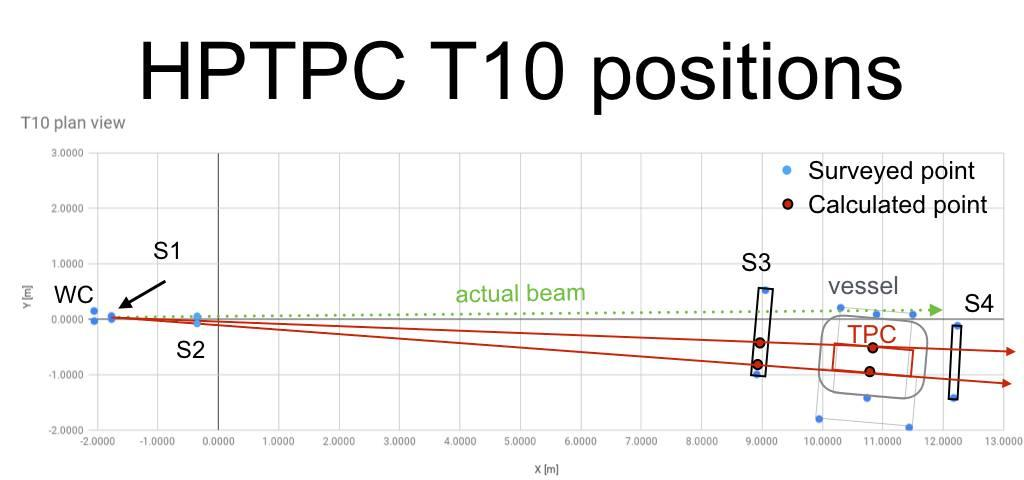
\includegraphics[width=1.0\linewidth]{files/Figures/T10Diagram.jpg}
    	\caption{Beam test configuration}
    		\label{fig:setup}
    \end{figure}
    The centre of the HPTPC Prototype was placed 13~m from the wire chamber at the beam entrance. 
    3 Time of Flight constituents, labeled S1 to S3, were placed upstream of the TPC, while the 4th, labeled S4, was placed directly downstream.
    Both the TPC and Time of Flight systems were placed at an off axis angle with resepct to the direction shown by the green arrow.
    Additionally, a variable number of blocks of acrylic moderator, shown in Figure~\ref{fig:modblocks}, were placed in the beamline, upstream of S1.
      \begin{figure}
      \centering
    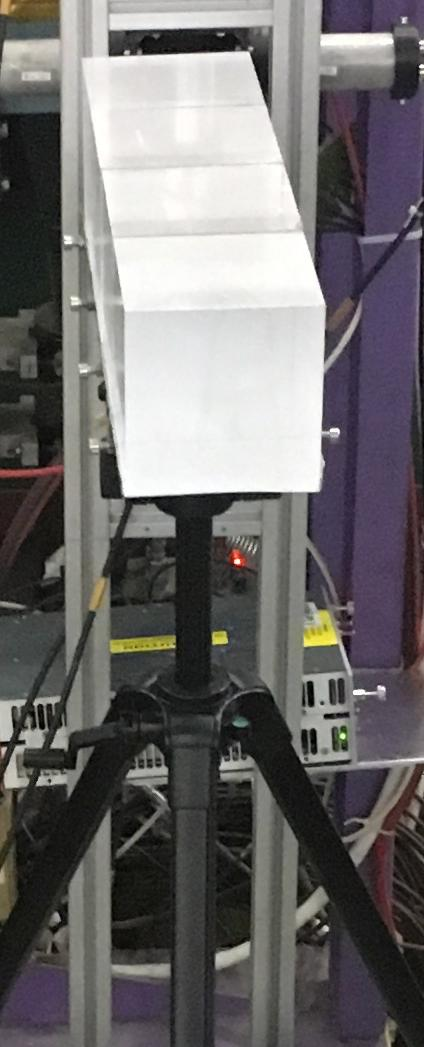
\includegraphics[width=0.2\linewidth]{files/Figures/ModeratorBlocks.jpg}
    	\caption{Acrylic Moderator Blocks}
    		\label{fig:modblocks}
    \end{figure}
    
    Moderator blocks were used in order to cause a spread in the incoming beam.
    The blocks cause protons to be spread through a larger angle than pions and other MIPs, increasing the off-axis proton pion ratio.
    The effect of this, together with placing the TPC and ToF systems off axis was to allow a measurement of protons with a lower pion background.
    This technique also had the effect of reducing the average momentum of the measured particles.
    Data were taken for 0, 1, 2, 3, and 4 moderator blocks in turn.
    
 
    
	\subsection{Upstream time instrumentation}
    The 

	\subsection{DsToF instrumentation}
	
    The downstream time of flight system, S4, consists of 10 bars of Nuvia plastic scintillator, which form the detector medium. Attached to either end of each of these scintillator bars is a 5" Hamamatsu R6594 photomultiplier tube. The bars are arranged in two rows of five, such that there is complete coverage for any beam particles incident upon the detector. Diagrams of the S4 wall, along with its dimensions are show in figure~\ref{fig:dstofFront} and~\ref{fig:dstofDiagonal}.
    
    The time resolution of the bars and PMTs was measured to be 1~ns. The spatial resolution of the bars and PMTs was measured to be 8.3~cm.
    
    \begin{figure}[ht]    
    	\begin{minipage}[t]{.48\textwidth}
    		\centering
    		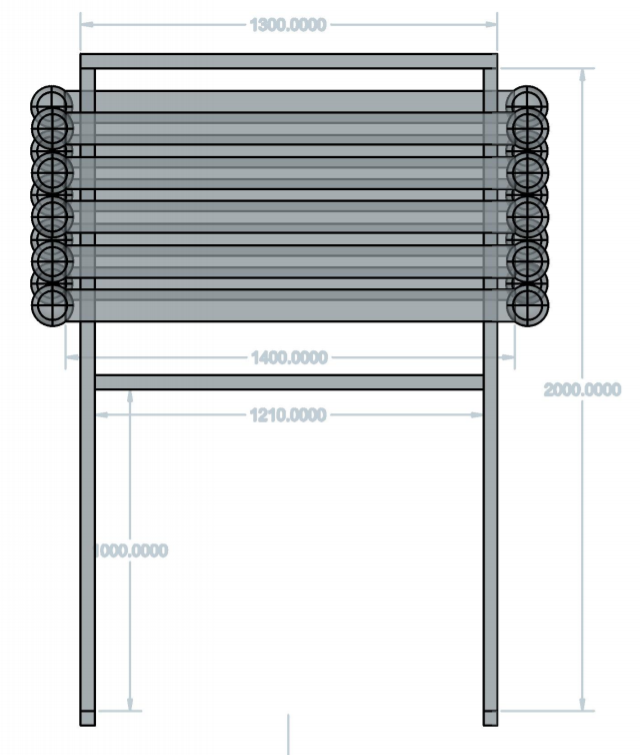
\includegraphics[width=0.6\linewidth]{files/Figures/dstofFront.png}
    		\caption{Front view of the downstream time of flight system}
    		\label{fig:dstofFront}
    	\end{minipage}
    	\hspace{0.3cm}
    	\begin{minipage}[t]{.48\textwidth}
    		\centering
    		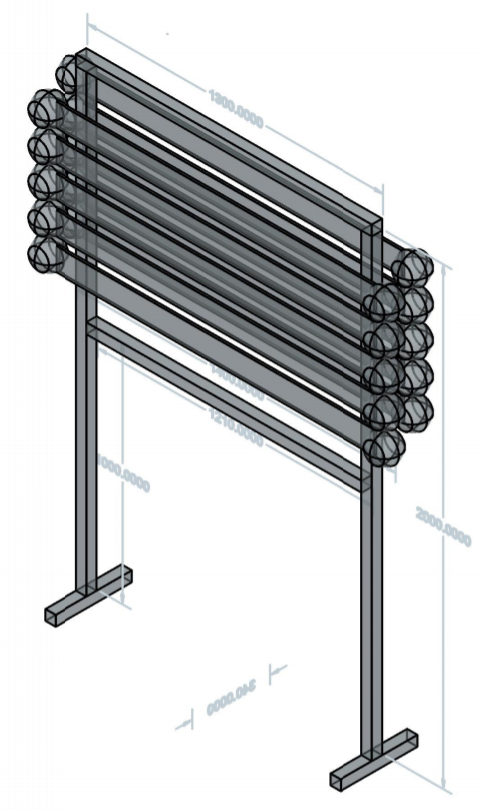
\includegraphics[width=0.45\linewidth]{files/Figures/dstofDiag.png}
    		\caption{Diagonal view of the downstream time of flight system showing more clearly the two rows of scintillator bars and photomultiplier tubes}
    		\label{fig:dstofDiagonal}
    	\end{minipage}
    \end{figure}
    
    All 20 of the photomultiplier tubes have their anode signals read out using NIM discriminators which are then fed into a time-to-digital converter. 
    
    A signal (i.e. an incident particle of any kind) in S4 was considered to have occurred if a signal was seen in both photomultiplier tubes on the same bar within 20~ns of each other.
    
    Additionally, a signal was also fed into the same time-to-digital converter whenever there was a coincidence between the S1 and S2 timing points. When calculating the time of flight of a given particle, this time of coincidence was used as first timing point.
    
	\subsection{Analysis methods -- $S_{4}$}

	Figure~\ref{fig:s4tof} shows the variation in the time of flight spectrum as recorded by the DsToF with a changing number of moderator blocks. This spectrum is formed from taking the difference in time between a coincidence being observed in the $S1$ and $S2$ timing points and a signal being recorded in $S4$ (the definition of an $S4$ signal is given above).
	
	\begin{figure}[h]
		\centering
		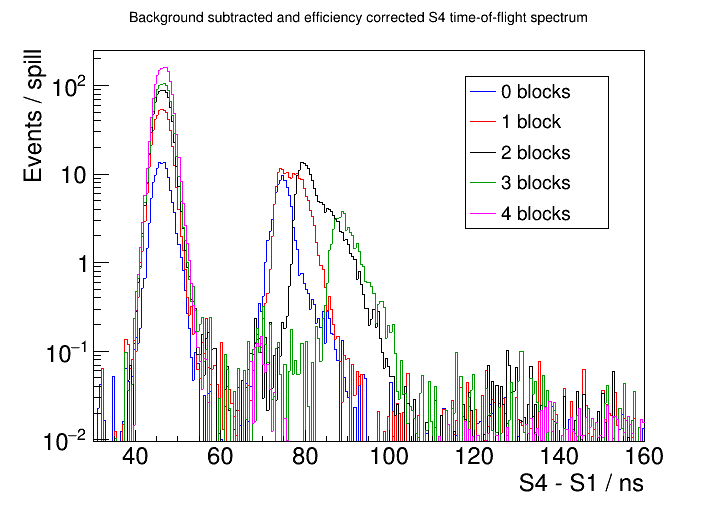
\includegraphics[width=0.7\linewidth]{files/Figures/s4ToF_axisAdj.png}
		\caption{$S_{4}$ time-of-flight spectra for varying numbers of moderator blocks. For all configurations, an exponentially falling background has been fitted and subtracted from the data. Additionally, the plot has also been corrected for the differing efficiencies of the various bars.}
		\label{fig:s4tof}	
	\end{figure}

	Furthermore, two corrections are applied to this measurement to give fig.~\ref{fig:s4tof}. Timing delays caused by cabling and equipment have to be taken into account. For this, a Gaussian is fitted to the peak caused by quicker particles and the mean of this is treated to have a value of $S4 - S1$ which corresponds to a particle traversing the distance between $S1$ and $S4$ at the speed of light. The other times are then shifted by the same amount.
	
	Additionally, the measurements are adjusted for the efficiency of each bar. The efficiency of each bar is calculated by taking the number of signal hits in coincidence with an $S1-S2$ signal in each bar and dividing by the total number of PMT hits in each bar which are themselves in coincidence with an $S1-S2$ signal. If we express the number of single PMT hits which are in coincidence with $S1-S2$ signal as $N_{1PMTcoins}$ and the number of 2 PMT signals in coincidence with an $S1-S2$ signal as $N_{2PMTcoins}$ then the efficiency is given by~(\ref{eq:barEff}).
	
	\begin{equation}
		\epsilon = \frac{N_{2PMTcoins}}{N_{2PMTcoins}+N_{1PMTcoins}}
		\label{eq:barEff}
	\end{equation}
	
	Using fig.~\ref{fig:s4tof} protons and MIPs are selected with timing cuts. These timing cuts are chosen by fitting a sum of signal and background functions to the time-of-flight spectra shown in figure~\ref{fig:s4tof}. The signal functions are taken to be Gaussians while the background is taken to be an exponential function. An example of this is shown in figure~\ref{fig:fitEx}.
	
	\begin{figure}[h]
		\centering
		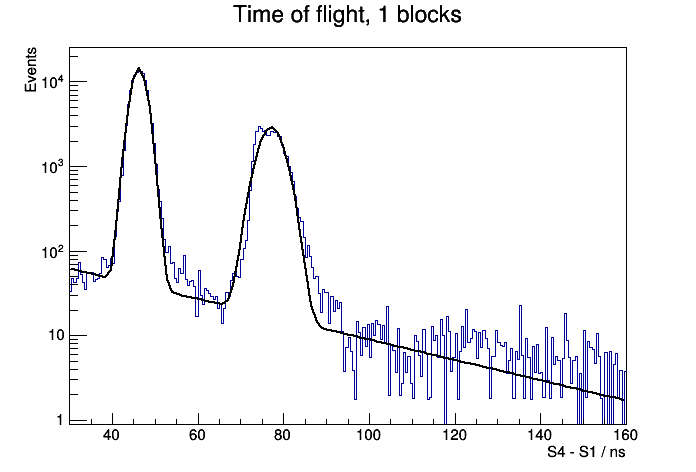
\includegraphics[width=0.6\textwidth]{files/Figures/1_dtof1d}
		\caption{Example of the time-of-flight spectrum observed in $S4$ with a combined signal and background function fitted (shown in black)}
		\label{fig:fitEx}
	\end{figure}

	To produce the data used in this analysis, an exponential background function is subtracted. The parameters for this function are taken from the combined signal and background function.
	
	\subsection{Analysis methods -- $S3$}
	
	
	\begin{figure}[h]
		\begin{adjustbox}{max totalsize={.9\textwidth}{.7\textheight},center}
			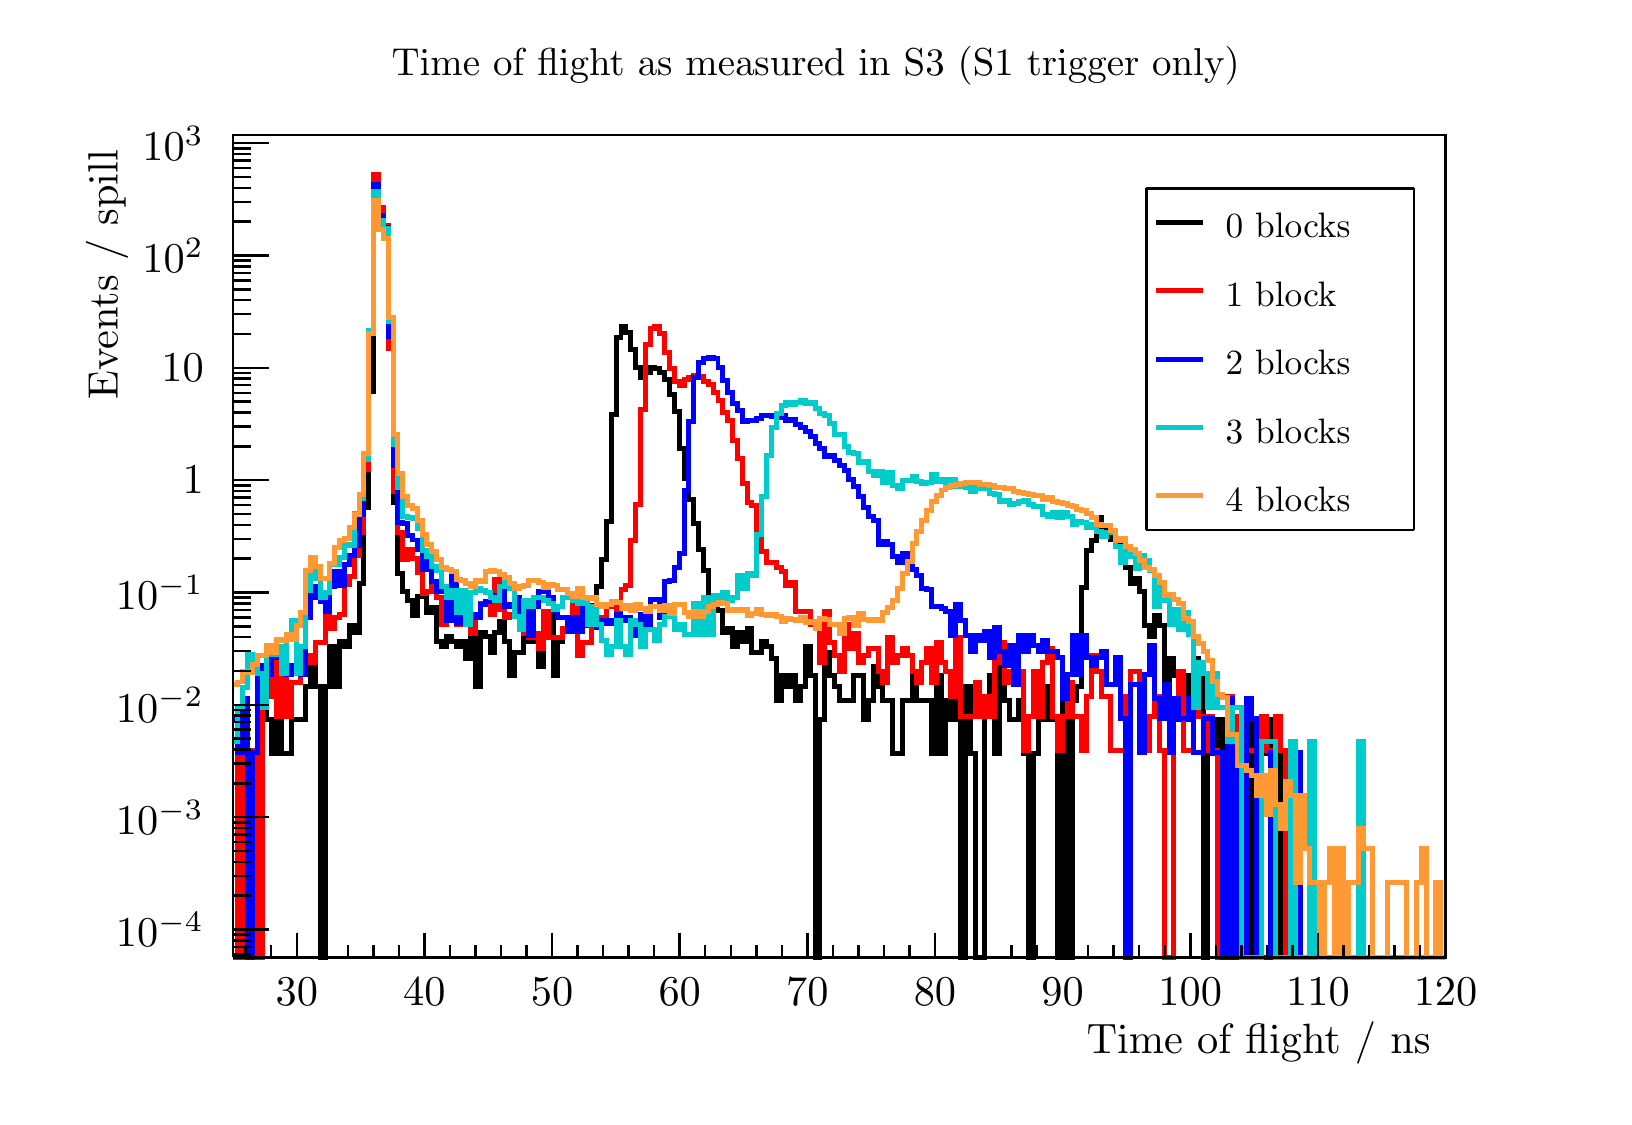
\begin{tikzpicture}
\pgfdeclareplotmark{cross} {
\pgfpathmoveto{\pgfpoint{-0.3\pgfplotmarksize}{\pgfplotmarksize}}
\pgfpathlineto{\pgfpoint{+0.3\pgfplotmarksize}{\pgfplotmarksize}}
\pgfpathlineto{\pgfpoint{+0.3\pgfplotmarksize}{0.3\pgfplotmarksize}}
\pgfpathlineto{\pgfpoint{+1\pgfplotmarksize}{0.3\pgfplotmarksize}}
\pgfpathlineto{\pgfpoint{+1\pgfplotmarksize}{-0.3\pgfplotmarksize}}
\pgfpathlineto{\pgfpoint{+0.3\pgfplotmarksize}{-0.3\pgfplotmarksize}}
\pgfpathlineto{\pgfpoint{+0.3\pgfplotmarksize}{-1.\pgfplotmarksize}}
\pgfpathlineto{\pgfpoint{-0.3\pgfplotmarksize}{-1.\pgfplotmarksize}}
\pgfpathlineto{\pgfpoint{-0.3\pgfplotmarksize}{-0.3\pgfplotmarksize}}
\pgfpathlineto{\pgfpoint{-1.\pgfplotmarksize}{-0.3\pgfplotmarksize}}
\pgfpathlineto{\pgfpoint{-1.\pgfplotmarksize}{0.3\pgfplotmarksize}}
\pgfpathlineto{\pgfpoint{-0.3\pgfplotmarksize}{0.3\pgfplotmarksize}}
\pgfpathclose
\pgfusepathqstroke
}
\pgfdeclareplotmark{cross*} {
\pgfpathmoveto{\pgfpoint{-0.3\pgfplotmarksize}{\pgfplotmarksize}}
\pgfpathlineto{\pgfpoint{+0.3\pgfplotmarksize}{\pgfplotmarksize}}
\pgfpathlineto{\pgfpoint{+0.3\pgfplotmarksize}{0.3\pgfplotmarksize}}
\pgfpathlineto{\pgfpoint{+1\pgfplotmarksize}{0.3\pgfplotmarksize}}
\pgfpathlineto{\pgfpoint{+1\pgfplotmarksize}{-0.3\pgfplotmarksize}}
\pgfpathlineto{\pgfpoint{+0.3\pgfplotmarksize}{-0.3\pgfplotmarksize}}
\pgfpathlineto{\pgfpoint{+0.3\pgfplotmarksize}{-1.\pgfplotmarksize}}
\pgfpathlineto{\pgfpoint{-0.3\pgfplotmarksize}{-1.\pgfplotmarksize}}
\pgfpathlineto{\pgfpoint{-0.3\pgfplotmarksize}{-0.3\pgfplotmarksize}}
\pgfpathlineto{\pgfpoint{-1.\pgfplotmarksize}{-0.3\pgfplotmarksize}}
\pgfpathlineto{\pgfpoint{-1.\pgfplotmarksize}{0.3\pgfplotmarksize}}
\pgfpathlineto{\pgfpoint{-0.3\pgfplotmarksize}{0.3\pgfplotmarksize}}
\pgfpathclose
\pgfusepathqfillstroke
}
\pgfdeclareplotmark{newstar} {
\pgfpathmoveto{\pgfqpoint{0pt}{\pgfplotmarksize}}
\pgfpathlineto{\pgfqpointpolar{44}{0.5\pgfplotmarksize}}
\pgfpathlineto{\pgfqpointpolar{18}{\pgfplotmarksize}}
\pgfpathlineto{\pgfqpointpolar{-20}{0.5\pgfplotmarksize}}
\pgfpathlineto{\pgfqpointpolar{-54}{\pgfplotmarksize}}
\pgfpathlineto{\pgfqpointpolar{-90}{0.5\pgfplotmarksize}}
\pgfpathlineto{\pgfqpointpolar{234}{\pgfplotmarksize}}
\pgfpathlineto{\pgfqpointpolar{198}{0.5\pgfplotmarksize}}
\pgfpathlineto{\pgfqpointpolar{162}{\pgfplotmarksize}}
\pgfpathlineto{\pgfqpointpolar{134}{0.5\pgfplotmarksize}}
\pgfpathclose
\pgfusepathqstroke
}
\pgfdeclareplotmark{newstar*} {
\pgfpathmoveto{\pgfqpoint{0pt}{\pgfplotmarksize}}
\pgfpathlineto{\pgfqpointpolar{44}{0.5\pgfplotmarksize}}
\pgfpathlineto{\pgfqpointpolar{18}{\pgfplotmarksize}}
\pgfpathlineto{\pgfqpointpolar{-20}{0.5\pgfplotmarksize}}
\pgfpathlineto{\pgfqpointpolar{-54}{\pgfplotmarksize}}
\pgfpathlineto{\pgfqpointpolar{-90}{0.5\pgfplotmarksize}}
\pgfpathlineto{\pgfqpointpolar{234}{\pgfplotmarksize}}
\pgfpathlineto{\pgfqpointpolar{198}{0.5\pgfplotmarksize}}
\pgfpathlineto{\pgfqpointpolar{162}{\pgfplotmarksize}}
\pgfpathlineto{\pgfqpointpolar{134}{0.5\pgfplotmarksize}}
\pgfpathclose
\pgfusepathqfillstroke
}
\definecolor{c}{rgb}{1,1,1};
\draw [color=c, fill=c] (0,0) rectangle (20,13.5632);
\draw [color=c, fill=c] (2.6,1.76322) rectangle (18,12.2069);
\definecolor{c}{rgb}{0,0,0};
\draw [c,line width=0.9] (2.6,1.76322) -- (2.6,12.2069) -- (18,12.2069) -- (18,1.76322) -- (2.6,1.76322);
\definecolor{c}{rgb}{1,1,1};
\draw [color=c, fill=c] (2.6,1.76322) rectangle (18,12.2069);
\definecolor{c}{rgb}{0,0,0};
\draw [c,line width=0.9] (2.6,1.76322) -- (2.6,12.2069) -- (18,12.2069) -- (18,1.76322) -- (2.6,1.76322);
\definecolor{c}{rgb}{0,0,0.6};
\draw [c,line width=0.9] (2.6,1.76322) -- (2.6616,1.76322) -- (2.6616,1.76322) -- (2.7232,1.76322) -- (2.7232,1.76322) -- (2.7848,1.76322) -- (2.7848,1.76322) -- (2.8464,1.76322) -- (2.8464,1.76322) -- (2.908,1.76322) -- (2.908,1.76322) --
 (2.9696,1.76322) -- (2.9696,1.76322) -- (3.0312,1.76322) -- (3.0312,1.76322) -- (3.0928,1.76322) -- (3.0928,1.76322) -- (3.1544,1.76322) -- (3.1544,1.76322) -- (3.216,1.76322) -- (3.216,1.76322) -- (3.2776,1.76322) -- (3.2776,1.76322) --
 (3.3392,1.76322) -- (3.3392,1.76322) -- (3.4008,1.76322) -- (3.4008,1.76322) -- (3.4624,1.76322) -- (3.4624,1.76322) -- (3.524,1.76322) -- (3.524,1.76322) -- (3.5856,1.76322) -- (3.5856,1.76322) -- (3.6472,1.76322) -- (3.6472,1.76322) --
 (3.7088,1.76322) -- (3.7088,1.76322) -- (3.7704,1.76322) -- (3.7704,1.76322) -- (3.832,1.76322) -- (3.832,1.76322) -- (3.8936,1.76322) -- (3.8936,1.76322) -- (3.9552,1.76322) -- (3.9552,1.76322) -- (4.0168,1.76322) -- (4.0168,1.76322) --
 (4.0784,1.76322) -- (4.0784,1.76322) -- (4.14,1.76322) -- (4.14,1.76322) -- (4.2016,1.76322) -- (4.2016,1.76322) -- (4.2632,1.76322) -- (4.2632,1.76322) -- (4.3248,1.76322) -- (4.3248,1.76322) -- (4.3864,1.76322) -- (4.3864,1.76322) --
 (4.448,1.76322) -- (4.448,1.76322) -- (4.5096,1.76322) -- (4.5096,1.76322) -- (4.5712,1.76322) -- (4.5712,1.76322) -- (4.6328,1.76322) -- (4.6328,1.76322) -- (4.6944,1.76322) -- (4.6944,1.76322) -- (4.756,1.76322) -- (4.756,1.76322) --
 (4.8176,1.76322) -- (4.8176,1.76322) -- (4.8792,1.76322) -- (4.8792,1.76322) -- (4.9408,1.76322) -- (4.9408,1.76322) -- (5.0024,1.76322) -- (5.0024,1.76322) -- (5.064,1.76322) -- (5.064,1.76322) -- (5.1256,1.76322) -- (5.1256,1.76322) --
 (5.1872,1.76322) -- (5.1872,1.76322) -- (5.2488,1.76322) -- (5.2488,1.76322) -- (5.3104,1.76322) -- (5.3104,1.76322) -- (5.372,1.76322) -- (5.372,1.76322) -- (5.4336,1.76322) -- (5.4336,1.76322) -- (5.4952,1.76322) -- (5.4952,1.76322) --
 (5.5568,1.76322) -- (5.5568,1.76322) -- (5.6184,1.76322) -- (5.6184,1.76322) -- (5.68,1.76322) -- (5.68,1.76322) -- (5.7416,1.76322) -- (5.7416,1.76322) -- (5.8032,1.76322) -- (5.8032,1.76322) -- (5.8648,1.76322) -- (5.8648,1.76322) --
 (5.9264,1.76322) -- (5.9264,1.76322) -- (5.988,1.76322) -- (5.988,1.76322) -- (6.0496,1.76322) -- (6.0496,1.76322) -- (6.1112,1.76322) -- (6.1112,1.76322) -- (6.1728,1.76322) -- (6.1728,1.76322) -- (6.2344,1.76322) -- (6.2344,1.76322) --
 (6.296,1.76322) -- (6.296,1.76322) -- (6.3576,1.76322) -- (6.3576,1.76322) -- (6.4192,1.76322) -- (6.4192,1.76322) -- (6.4808,1.76322) -- (6.4808,1.76322) -- (6.5424,1.76322) -- (6.5424,1.76322) -- (6.604,1.76322) -- (6.604,1.76322) --
 (6.6656,1.76322) -- (6.6656,1.76322) -- (6.7272,1.76322) -- (6.7272,1.76322) -- (6.7888,1.76322) -- (6.7888,1.76322) -- (6.8504,1.76322) -- (6.8504,1.76322) -- (6.912,1.76322) -- (6.912,1.76322) -- (6.9736,1.76322) -- (6.9736,1.76322) --
 (7.0352,1.76322) -- (7.0352,1.76322) -- (7.0968,1.76322) -- (7.0968,1.76322) -- (7.1584,1.76322) -- (7.1584,1.76322) -- (7.22,1.76322) -- (7.22,1.76322) -- (7.2816,1.76322) -- (7.2816,1.76322) -- (7.3432,1.76322) -- (7.3432,1.76322) --
 (7.4048,1.76322) -- (7.4048,1.76322) -- (7.4664,1.76322) -- (7.4664,1.76322) -- (7.528,1.76322) -- (7.528,1.76322) -- (7.5896,1.76322) -- (7.5896,1.76322) -- (7.6512,1.76322) -- (7.6512,1.76322) -- (7.7128,1.76322) -- (7.7128,1.76322) --
 (7.7744,1.76322) -- (7.7744,1.76322) -- (7.836,1.76322) -- (7.836,1.76322) -- (7.8976,1.76322) -- (7.8976,1.76322) -- (7.9592,1.76322) -- (7.9592,1.76322) -- (8.0208,1.76322) -- (8.0208,1.76322) -- (8.0824,1.76322) -- (8.0824,1.76322) --
 (8.144,1.76322) -- (8.144,1.76322) -- (8.2056,1.76322) -- (8.2056,1.76322) -- (8.2672,1.76322) -- (8.2672,1.76322) -- (8.3288,1.76322) -- (8.3288,1.76322) -- (8.3904,1.76322) -- (8.3904,1.76322) -- (8.452,1.76322) -- (8.452,1.76322) --
 (8.5136,1.76322) -- (8.5136,1.76322) -- (8.5752,1.76322) -- (8.5752,1.76322) -- (8.6368,1.76322) -- (8.6368,1.76322) -- (8.6984,1.76322) -- (8.6984,1.76322) -- (8.76,1.76322) -- (8.76,1.76322) -- (8.8216,1.76322) -- (8.8216,1.76322) --
 (8.8832,1.76322) -- (8.8832,1.76322) -- (8.9448,1.76322) -- (8.9448,1.76322) -- (9.0064,1.76322) -- (9.0064,1.76322) -- (9.068,1.76322) -- (9.068,1.76322) -- (9.1296,1.76322) -- (9.1296,1.76322) -- (9.1912,1.76322) -- (9.1912,1.76322) --
 (9.2528,1.76322) -- (9.2528,1.76322) -- (9.3144,1.76322) -- (9.3144,1.76322) -- (9.376,1.76322) -- (9.376,1.76322) -- (9.4376,1.76322) -- (9.4376,1.76322) -- (9.4992,1.76322) -- (9.4992,1.76322) -- (9.5608,1.76322) -- (9.5608,1.76322) --
 (9.6224,1.76322) -- (9.6224,1.76322) -- (9.684,1.76322) -- (9.684,1.76322) -- (9.7456,1.76322) -- (9.7456,1.76322) -- (9.8072,1.76322) -- (9.8072,1.76322) -- (9.8688,1.76322) -- (9.8688,1.76322) -- (9.9304,1.76322) -- (9.9304,1.76322) --
 (9.992,1.76322) -- (9.992,1.76322) -- (10.0536,1.76322) -- (10.0536,1.76322) -- (10.1152,1.76322) -- (10.1152,1.76322) -- (10.1768,1.76322) -- (10.1768,1.76322) -- (10.2384,1.76322) -- (10.2384,1.76322) -- (10.3,1.76322) -- (10.3,1.76322) --
 (10.3616,1.76322) -- (10.3616,1.76322) -- (10.4232,1.76322) -- (10.4232,1.76322) -- (10.4848,1.76322) -- (10.4848,1.76322) -- (10.5464,1.76322) -- (10.5464,1.76322) -- (10.608,1.76322) -- (10.608,1.76322) -- (10.6696,1.76322) -- (10.6696,1.76322) --
 (10.7312,1.76322) -- (10.7312,1.76322) -- (10.7928,1.76322) -- (10.7928,1.76322) -- (10.8544,1.76322) -- (10.8544,1.76322) -- (10.916,1.76322) -- (10.916,1.76322) -- (10.9776,1.76322) -- (10.9776,1.76322) -- (11.0392,1.76322) -- (11.0392,1.76322) --
 (11.1008,1.76322) -- (11.1008,1.76322) -- (11.1624,1.76322) -- (11.1624,1.76322) -- (11.224,1.76322) -- (11.224,1.76322) -- (11.2856,1.76322) -- (11.2856,1.76322) -- (11.3472,1.76322) -- (11.3472,1.76322) -- (11.4088,1.76322) -- (11.4088,1.76322) --
 (11.4704,1.76322) -- (11.4704,1.76322) -- (11.532,1.76322) -- (11.532,1.76322) -- (11.5936,1.76322) -- (11.5936,1.76322) -- (11.6552,1.76322) -- (11.6552,1.76322) -- (11.7168,1.76322) -- (11.7168,1.76322) -- (11.7784,1.76322) -- (11.7784,1.76322) --
 (11.84,1.76322) -- (11.84,1.76322) -- (11.9016,1.76322) -- (11.9016,1.76322) -- (11.9632,1.76322) -- (11.9632,1.76322) -- (12.0248,1.76322) -- (12.0248,1.76322) -- (12.0864,1.76322) -- (12.0864,1.76322) -- (12.148,1.76322) -- (12.148,1.76322) --
 (12.2096,1.76322) -- (12.2096,1.76322) -- (12.2712,1.76322) -- (12.2712,1.76322) -- (12.3328,1.76322) -- (12.3328,1.76322) -- (12.3944,1.76322) -- (12.3944,1.76322) -- (12.456,1.76322) -- (12.456,1.76322) -- (12.5176,1.76322) -- (12.5176,1.76322) --
 (12.5792,1.76322) -- (12.5792,1.76322) -- (12.6408,1.76322) -- (12.6408,1.76322) -- (12.7024,1.76322) -- (12.7024,1.76322) -- (12.764,1.76322) -- (12.764,1.76322) -- (12.8256,1.76322) -- (12.8256,1.76322) -- (12.8872,1.76322) -- (12.8872,1.76322) --
 (12.9488,1.76322) -- (12.9488,1.76322) -- (13.0104,1.76322) -- (13.0104,1.76322) -- (13.072,1.76322) -- (13.072,1.76322) -- (13.1336,1.76322) -- (13.1336,1.76322) -- (13.1952,1.76322) -- (13.1952,1.76322) -- (13.2568,1.76322) -- (13.2568,1.76322) --
 (13.3184,1.76322) -- (13.3184,1.76322) -- (13.38,1.76322) -- (13.38,1.76322) -- (13.4416,1.76322) -- (13.4416,1.76322) -- (13.5032,1.76322) -- (13.5032,1.76322) -- (13.5648,1.76322) -- (13.5648,1.76322) -- (13.6264,1.76322) -- (13.6264,1.76322) --
 (13.688,1.76322) -- (13.688,1.76322) -- (13.7496,1.76322) -- (13.7496,1.76322) -- (13.8112,1.76322) -- (13.8112,1.76322) -- (13.8728,1.76322) -- (13.8728,1.76322) -- (13.9344,1.76322) -- (13.9344,1.76322) -- (13.996,1.76322) -- (13.996,1.76322) --
 (14.0576,1.76322) -- (14.0576,1.76322) -- (14.1192,1.76322) -- (14.1192,1.76322) -- (14.1808,1.76322) -- (14.1808,1.76322) -- (14.2424,1.76322) -- (14.2424,1.76322) -- (14.304,1.76322) -- (14.304,1.76322) -- (14.3656,1.76322) -- (14.3656,1.76322) --
 (14.4272,1.76322) -- (14.4272,1.76322) -- (14.4888,1.76322) -- (14.4888,1.76322) -- (14.5504,1.76322) -- (14.5504,1.76322) -- (14.612,1.76322) -- (14.612,1.76322) -- (14.6736,1.76322) -- (14.6736,1.76322) -- (14.7352,1.76322) -- (14.7352,1.76322) --
 (14.7968,1.76322) -- (14.7968,1.76322) -- (14.8584,1.76322) -- (14.8584,1.76322) -- (14.92,1.76322) -- (14.92,1.76322) -- (14.9816,1.76322) -- (14.9816,1.76322) -- (15.0432,1.76322) -- (15.0432,1.76322) -- (15.1048,1.76322) -- (15.1048,1.76322) --
 (15.1664,1.76322) -- (15.1664,1.76322) -- (15.228,1.76322) -- (15.228,1.76322) -- (15.2896,1.76322) -- (15.2896,1.76322) -- (15.3512,1.76322) -- (15.3512,1.76322) -- (15.4128,1.76322) -- (15.4128,1.76322) -- (15.4744,1.76322) -- (15.4744,1.76322) --
 (15.536,1.76322) -- (15.536,1.76322) -- (15.5976,1.76322) -- (15.5976,1.76322) -- (15.6592,1.76322) -- (15.6592,1.76322) -- (15.7208,1.76322) -- (15.7208,1.76322) -- (15.7824,1.76322) -- (15.7824,1.76322) -- (15.844,1.76322) -- (15.844,1.76322) --
 (15.9056,1.76322) -- (15.9056,1.76322) -- (15.9672,1.76322) -- (15.9672,1.76322) -- (16.0288,1.76322) -- (16.0288,1.76322) -- (16.0904,1.76322) -- (16.0904,1.76322) -- (16.152,1.76322) -- (16.152,1.76322) -- (16.2136,1.76322) -- (16.2136,1.76322) --
 (16.2752,1.76322) -- (16.2752,1.76322) -- (16.3368,1.76322) -- (16.3368,1.76322) -- (16.3984,1.76322) -- (16.3984,1.76322) -- (16.46,1.76322) -- (16.46,1.76322) -- (16.5216,1.76322) -- (16.5216,1.76322) -- (16.5832,1.76322) -- (16.5832,1.76322) --
 (16.6448,1.76322) -- (16.6448,1.76322) -- (16.7064,1.76322) -- (16.7064,1.76322) -- (16.768,1.76322) -- (16.768,1.76322) -- (16.8296,1.76322) -- (16.8296,1.76322) -- (16.8912,1.76322) -- (16.8912,1.76322) -- (16.9528,1.76322) -- (16.9528,1.76322) --
 (17.0144,1.76322) -- (17.0144,1.76322) -- (17.076,1.76322) -- (17.076,1.76322) -- (17.1376,1.76322) -- (17.1376,1.76322) -- (17.1992,1.76322) -- (17.1992,1.76322) -- (17.2608,1.76322) -- (17.2608,1.76322) -- (17.3224,1.76322) -- (17.3224,1.76322) --
 (17.384,1.76322) -- (17.384,1.76322) -- (17.4456,1.76322) -- (17.4456,1.76322) -- (17.5072,1.76322) -- (17.5072,1.76322) -- (17.5688,1.76322) -- (17.5688,1.76322) -- (17.6304,1.76322) -- (17.6304,1.76322) -- (17.692,1.76322) -- (17.692,1.76322) --
 (17.7536,1.76322) -- (17.7536,1.76322) -- (17.8152,1.76322) -- (17.8152,1.76322) -- (17.8768,1.76322) -- (17.8768,1.76322) -- (17.9384,1.76322) -- (17.9384,1.76322) -- (18,1.76322);
\definecolor{c}{rgb}{0,0,0};
\draw [c,line width=0.9] (2.6,1.76322) -- (18,1.76322);
\draw [anchor= east] (18,0.678161) node[scale=1.5317, color=c, rotate=0]{ Time of flight / ns};
\draw [c,line width=0.9] (3.41053,2.07653) -- (3.41053,1.76322);
\draw [c,line width=0.9] (3.73474,1.91987) -- (3.73474,1.76322);
\draw [c,line width=0.9] (4.05895,1.91987) -- (4.05895,1.76322);
\draw [c,line width=0.9] (4.38316,1.91987) -- (4.38316,1.76322);
\draw [c,line width=0.9] (4.70737,1.91987) -- (4.70737,1.76322);
\draw [c,line width=0.9] (5.03158,2.07653) -- (5.03158,1.76322);
\draw [c,line width=0.9] (5.35579,1.91987) -- (5.35579,1.76322);
\draw [c,line width=0.9] (5.68,1.91987) -- (5.68,1.76322);
\draw [c,line width=0.9] (6.00421,1.91987) -- (6.00421,1.76322);
\draw [c,line width=0.9] (6.32842,1.91987) -- (6.32842,1.76322);
\draw [c,line width=0.9] (6.65263,2.07653) -- (6.65263,1.76322);
\draw [c,line width=0.9] (6.97684,1.91987) -- (6.97684,1.76322);
\draw [c,line width=0.9] (7.30105,1.91987) -- (7.30105,1.76322);
\draw [c,line width=0.9] (7.62526,1.91987) -- (7.62526,1.76322);
\draw [c,line width=0.9] (7.94947,1.91987) -- (7.94947,1.76322);
\draw [c,line width=0.9] (8.27368,2.07653) -- (8.27368,1.76322);
\draw [c,line width=0.9] (8.59789,1.91987) -- (8.59789,1.76322);
\draw [c,line width=0.9] (8.9221,1.91987) -- (8.9221,1.76322);
\draw [c,line width=0.9] (9.24632,1.91987) -- (9.24632,1.76322);
\draw [c,line width=0.9] (9.57053,1.91987) -- (9.57053,1.76322);
\draw [c,line width=0.9] (9.89474,2.07653) -- (9.89474,1.76322);
\draw [c,line width=0.9] (10.2189,1.91987) -- (10.2189,1.76322);
\draw [c,line width=0.9] (10.5432,1.91987) -- (10.5432,1.76322);
\draw [c,line width=0.9] (10.8674,1.91987) -- (10.8674,1.76322);
\draw [c,line width=0.9] (11.1916,1.91987) -- (11.1916,1.76322);
\draw [c,line width=0.9] (11.5158,2.07653) -- (11.5158,1.76322);
\draw [c,line width=0.9] (11.84,1.91987) -- (11.84,1.76322);
\draw [c,line width=0.9] (12.1642,1.91987) -- (12.1642,1.76322);
\draw [c,line width=0.9] (12.4884,1.91987) -- (12.4884,1.76322);
\draw [c,line width=0.9] (12.8126,1.91987) -- (12.8126,1.76322);
\draw [c,line width=0.9] (13.1368,2.07653) -- (13.1368,1.76322);
\draw [c,line width=0.9] (13.4611,1.91987) -- (13.4611,1.76322);
\draw [c,line width=0.9] (13.7853,1.91987) -- (13.7853,1.76322);
\draw [c,line width=0.9] (14.1095,1.91987) -- (14.1095,1.76322);
\draw [c,line width=0.9] (14.4337,1.91987) -- (14.4337,1.76322);
\draw [c,line width=0.9] (14.7579,2.07653) -- (14.7579,1.76322);
\draw [c,line width=0.9] (15.0821,1.91987) -- (15.0821,1.76322);
\draw [c,line width=0.9] (15.4063,1.91987) -- (15.4063,1.76322);
\draw [c,line width=0.9] (15.7305,1.91987) -- (15.7305,1.76322);
\draw [c,line width=0.9] (16.0547,1.91987) -- (16.0547,1.76322);
\draw [c,line width=0.9] (16.3789,2.07653) -- (16.3789,1.76322);
\draw [c,line width=0.9] (16.7032,1.91987) -- (16.7032,1.76322);
\draw [c,line width=0.9] (17.0274,1.91987) -- (17.0274,1.76322);
\draw [c,line width=0.9] (17.3516,1.91987) -- (17.3516,1.76322);
\draw [c,line width=0.9] (17.6758,1.91987) -- (17.6758,1.76322);
\draw [c,line width=0.9] (18,2.07653) -- (18,1.76322);
\draw [c,line width=0.9] (3.41053,2.07653) -- (3.41053,1.76322);
\draw [c,line width=0.9] (3.08632,1.91987) -- (3.08632,1.76322);
\draw [c,line width=0.9] (2.76211,1.91987) -- (2.76211,1.76322);
\draw [anchor=base] (3.41053,1.15287) node[scale=1.5317, color=c, rotate=0]{30};
\draw [anchor=base] (5.03158,1.15287) node[scale=1.5317, color=c, rotate=0]{40};
\draw [anchor=base] (6.65263,1.15287) node[scale=1.5317, color=c, rotate=0]{50};
\draw [anchor=base] (8.27368,1.15287) node[scale=1.5317, color=c, rotate=0]{60};
\draw [anchor=base] (9.89474,1.15287) node[scale=1.5317, color=c, rotate=0]{70};
\draw [anchor=base] (11.5158,1.15287) node[scale=1.5317, color=c, rotate=0]{80};
\draw [anchor=base] (13.1368,1.15287) node[scale=1.5317, color=c, rotate=0]{90};
\draw [anchor=base] (14.7579,1.15287) node[scale=1.5317, color=c, rotate=0]{100};
\draw [anchor=base] (16.3789,1.15287) node[scale=1.5317, color=c, rotate=0]{110};
\draw [anchor=base] (18,1.15287) node[scale=1.5317, color=c, rotate=0]{120};
\draw [c,line width=0.9] (2.6,1.76322) -- (2.6,12.2069);
\draw [anchor= east] (1,12.2069) node[scale=1.5317, color=c, rotate=90]{ Events / spill};
\draw [c,line width=0.9] (2.831,1.80116) -- (2.6,1.80116);
\draw [c,line width=0.9] (2.831,1.89666) -- (2.6,1.89666);
\draw [c,line width=0.9] (2.831,1.97939) -- (2.6,1.97939);
\draw [c,line width=0.9] (2.831,2.05235) -- (2.6,2.05235);
\draw [c,line width=0.9] (3.062,2.11763) -- (2.6,2.11763);
\draw [anchor= east] (2.42,2.11763) node[scale=1.5317, color=c, rotate=0]{$10^{-4}$};
\draw [c,line width=0.9] (2.831,2.54704) -- (2.6,2.54704);
\draw [c,line width=0.9] (2.831,2.79823) -- (2.6,2.79823);
\draw [c,line width=0.9] (2.831,2.97645) -- (2.6,2.97645);
\draw [c,line width=0.9] (2.831,3.11469) -- (2.6,3.11469);
\draw [c,line width=0.9] (2.831,3.22764) -- (2.6,3.22764);
\draw [c,line width=0.9] (2.831,3.32314) -- (2.6,3.32314);
\draw [c,line width=0.9] (2.831,3.40586) -- (2.6,3.40586);
\draw [c,line width=0.9] (2.831,3.47883) -- (2.6,3.47883);
\draw [c,line width=0.9] (3.062,3.5441) -- (2.6,3.5441);
\draw [anchor= east] (2.42,3.5441) node[scale=1.5317, color=c, rotate=0]{$10^{-3}$};
\draw [c,line width=0.9] (2.831,3.97352) -- (2.6,3.97352);
\draw [c,line width=0.9] (2.831,4.22471) -- (2.6,4.22471);
\draw [c,line width=0.9] (2.831,4.40293) -- (2.6,4.40293);
\draw [c,line width=0.9] (2.831,4.54117) -- (2.6,4.54117);
\draw [c,line width=0.9] (2.831,4.65412) -- (2.6,4.65412);
\draw [c,line width=0.9] (2.831,4.74962) -- (2.6,4.74962);
\draw [c,line width=0.9] (2.831,4.83234) -- (2.6,4.83234);
\draw [c,line width=0.9] (2.831,4.90531) -- (2.6,4.90531);
\draw [c,line width=0.9] (3.062,4.97058) -- (2.6,4.97058);
\draw [anchor= east] (2.42,4.97058) node[scale=1.5317, color=c, rotate=0]{$10^{-2}$};
\draw [c,line width=0.9] (2.831,5.39999) -- (2.6,5.39999);
\draw [c,line width=0.9] (2.831,5.65118) -- (2.6,5.65118);
\draw [c,line width=0.9] (2.831,5.82941) -- (2.6,5.82941);
\draw [c,line width=0.9] (2.831,5.96765) -- (2.6,5.96765);
\draw [c,line width=0.9] (2.831,6.0806) -- (2.6,6.0806);
\draw [c,line width=0.9] (2.831,6.17609) -- (2.6,6.17609);
\draw [c,line width=0.9] (2.831,6.25882) -- (2.6,6.25882);
\draw [c,line width=0.9] (2.831,6.33179) -- (2.6,6.33179);
\draw [c,line width=0.9] (3.062,6.39706) -- (2.6,6.39706);
\draw [anchor= east] (2.42,6.39706) node[scale=1.5317, color=c, rotate=0]{$10^{-1}$};
\draw [c,line width=0.9] (2.831,6.82647) -- (2.6,6.82647);
\draw [c,line width=0.9] (2.831,7.07766) -- (2.6,7.07766);
\draw [c,line width=0.9] (2.831,7.25588) -- (2.6,7.25588);
\draw [c,line width=0.9] (2.831,7.39412) -- (2.6,7.39412);
\draw [c,line width=0.9] (2.831,7.50707) -- (2.6,7.50707);
\draw [c,line width=0.9] (2.831,7.60257) -- (2.6,7.60257);
\draw [c,line width=0.9] (2.831,7.6853) -- (2.6,7.6853);
\draw [c,line width=0.9] (2.831,7.75826) -- (2.6,7.75826);
\draw [c,line width=0.9] (3.062,7.82354) -- (2.6,7.82354);
\draw [anchor= east] (2.42,7.82354) node[scale=1.5317, color=c, rotate=0]{1};
\draw [c,line width=0.9] (2.831,8.25295) -- (2.6,8.25295);
\draw [c,line width=0.9] (2.831,8.50414) -- (2.6,8.50414);
\draw [c,line width=0.9] (2.831,8.68236) -- (2.6,8.68236);
\draw [c,line width=0.9] (2.831,8.8206) -- (2.6,8.8206);
\draw [c,line width=0.9] (2.831,8.93355) -- (2.6,8.93355);
\draw [c,line width=0.9] (2.831,9.02905) -- (2.6,9.02905);
\draw [c,line width=0.9] (2.831,9.11177) -- (2.6,9.11177);
\draw [c,line width=0.9] (2.831,9.18474) -- (2.6,9.18474);
\draw [c,line width=0.9] (3.062,9.25001) -- (2.6,9.25001);
\draw [anchor= east] (2.42,9.25001) node[scale=1.5317, color=c, rotate=0]{10};
\draw [c,line width=0.9] (2.831,9.67943) -- (2.6,9.67943);
\draw [c,line width=0.9] (2.831,9.93062) -- (2.6,9.93062);
\draw [c,line width=0.9] (2.831,10.1088) -- (2.6,10.1088);
\draw [c,line width=0.9] (2.831,10.2471) -- (2.6,10.2471);
\draw [c,line width=0.9] (2.831,10.36) -- (2.6,10.36);
\draw [c,line width=0.9] (2.831,10.4555) -- (2.6,10.4555);
\draw [c,line width=0.9] (2.831,10.5383) -- (2.6,10.5383);
\draw [c,line width=0.9] (2.831,10.6112) -- (2.6,10.6112);
\draw [c,line width=0.9] (3.062,10.6765) -- (2.6,10.6765);
\draw [anchor= east] (2.42,10.6765) node[scale=1.5317, color=c, rotate=0]{$10^{2}$};
\draw [c,line width=0.9] (2.831,11.1059) -- (2.6,11.1059);
\draw [c,line width=0.9] (2.831,11.3571) -- (2.6,11.3571);
\draw [c,line width=0.9] (2.831,11.5353) -- (2.6,11.5353);
\draw [c,line width=0.9] (2.831,11.6736) -- (2.6,11.6736);
\draw [c,line width=0.9] (2.831,11.7865) -- (2.6,11.7865);
\draw [c,line width=0.9] (2.831,11.882) -- (2.6,11.882);
\draw [c,line width=0.9] (2.831,11.9647) -- (2.6,11.9647);
\draw [c,line width=0.9] (2.831,12.0377) -- (2.6,12.0377);
\draw [c,line width=0.9] (3.062,12.103) -- (2.6,12.103);
\draw [anchor= east] (2.42,12.103) node[scale=1.5317, color=c, rotate=0]{$10^{3}$};
\draw [c,line width=1.8] (2.6,1.76322) -- (2.6616,1.76322) -- (2.6616,1.76322) -- (2.7232,1.76322) -- (2.7232,1.76322) -- (2.7848,1.76322) -- (2.7848,1.76322) -- (2.8464,1.76322) -- (2.8464,4.3484) -- (2.908,4.3484) -- (2.908,4.3484) --
 (2.9696,4.3484) -- (2.9696,5.02901) -- (3.0312,5.02901) -- (3.0312,4.77782) -- (3.0928,4.77782) -- (3.0928,4.3484) -- (3.1544,4.3484) -- (3.1544,5.45842) -- (3.216,5.45842) -- (3.216,4.3484) -- (3.2776,4.3484) -- (3.2776,4.3484) -- (3.3392,4.3484)
 -- (3.3392,4.77782) -- (3.4008,4.77782) -- (3.4008,4.77782) -- (3.4624,4.77782) -- (3.4624,4.77782) -- (3.524,4.77782) -- (3.524,5.20723) -- (3.5856,5.20723) -- (3.5856,5.45842) -- (3.6472,5.45842) -- (3.6472,5.20723) -- (3.7088,5.20723) --
 (3.7088,1.76322) -- (3.7704,1.76322) -- (3.7704,5.20723) -- (3.832,5.20723) -- (3.832,5.70961) -- (3.8936,5.70961) -- (3.8936,5.20723) -- (3.9552,5.20723) -- (3.9552,5.77488) -- (4.0168,5.77488) -- (4.0168,5.70961) -- (4.0784,5.70961) --
 (4.0784,5.98333) -- (4.14,5.98333) -- (4.14,5.88783) -- (4.2016,5.88783) -- (4.2016,6.51453) -- (4.2632,6.51453) -- (4.2632,7.47685) -- (4.3248,7.47685) -- (4.3248,8.94591) -- (4.3864,8.94591) -- (4.3864,11.3173) -- (4.448,11.3173) --
 (4.448,11.2886) -- (4.5096,11.2886) -- (4.5096,10.9646) -- (4.5712,10.9646) -- (4.5712,9.73246) -- (4.6328,9.73246) -- (4.6328,7.54093) -- (4.6944,7.54093) -- (4.6944,6.63371) -- (4.756,6.63371) -- (4.756,6.41274) -- (4.8176,6.41274) --
 (4.8176,6.29088) -- (4.8792,6.29088) -- (4.8792,6.10361) -- (4.9408,6.10361) -- (4.9408,6.34253) -- (5.0024,6.34253) -- (5.0024,6.36683) -- (5.064,6.36683) -- (5.064,6.13902) -- (5.1256,6.13902) -- (5.1256,6.20429) -- (5.1872,6.20429) --
 (5.1872,5.77488) -- (5.2488,5.77488) -- (5.2488,5.70961) -- (5.3104,5.70961) -- (5.3104,5.83393) -- (5.372,5.83393) -- (5.372,5.77488) -- (5.4336,5.77488) -- (5.4336,5.70961) -- (5.4952,5.70961) -- (5.4952,5.77488) -- (5.5568,5.77488) --
 (5.5568,5.55392) -- (5.6184,5.55392) -- (5.6184,5.88783) -- (5.68,5.88783) -- (5.68,5.20723) -- (5.7416,5.20723) -- (5.7416,5.88783) -- (5.8032,5.88783) -- (5.8032,5.83393) -- (5.8648,5.83393) -- (5.8648,5.63664) -- (5.9264,5.63664) --
 (5.9264,5.88783) -- (5.988,5.88783) -- (5.988,6.02607) -- (6.0496,6.02607) -- (6.0496,5.77488) -- (6.1112,5.77488) -- (6.1112,5.34547) -- (6.1728,5.34547) -- (6.1728,5.63664) -- (6.2344,5.63664) -- (6.2344,5.63664) -- (6.296,5.63664) --
 (6.296,5.93742) -- (6.3576,5.93742) -- (6.3576,5.77488) -- (6.4192,5.77488) -- (6.4192,5.83393) -- (6.4808,5.83393) -- (6.4808,5.45842) -- (6.5424,5.45842) -- (6.5424,5.93742) -- (6.604,5.93742) -- (6.604,6.13902) -- (6.6656,6.13902) --
 (6.6656,5.34547) -- (6.7272,5.34547) -- (6.7272,5.77488) -- (6.7888,5.77488) -- (6.7888,5.93742) -- (6.8504,5.93742) -- (6.8504,6.02607) -- (6.912,6.02607) -- (6.912,6.10361) -- (6.9736,6.10361) -- (6.9736,5.93742) -- (7.0352,5.93742) --
 (7.0352,6.06605) -- (7.0968,6.06605) -- (7.0968,5.98333) -- (7.1584,5.98333) -- (7.1584,6.23452) -- (7.22,6.23452) -- (7.22,6.4758) -- (7.2816,6.4758) -- (7.2816,6.81962) -- (7.3432,6.81962) -- (7.3432,7.29331) -- (7.4048,7.29331) --
 (7.4048,8.65333) -- (7.4664,8.65333) -- (7.4664,9.63449) -- (7.528,9.63449) -- (7.528,9.77774) -- (7.5896,9.77774) -- (7.5896,9.69411) -- (7.6512,9.69411) -- (7.6512,9.4784) -- (7.7128,9.4784) -- (7.7128,9.25476) -- (7.7744,9.25476) --
 (7.7744,9.13351) -- (7.836,9.13351) -- (7.836,9.19126) -- (7.8976,9.19126) -- (7.8976,9.25611) -- (7.9592,9.25611) -- (7.9592,9.24386) -- (8.0208,9.24386) -- (8.0208,9.19276) -- (8.0824,9.19276) -- (8.0824,9.10292) -- (8.144,9.10292) --
 (8.144,8.91043) -- (8.2056,8.91043) -- (8.2056,8.69804) -- (8.2672,8.69804) -- (8.2672,8.22272) -- (8.3288,8.22272) -- (8.3288,7.83922) -- (8.3904,7.83922) -- (8.3904,7.58247) -- (8.452,7.58247) -- (8.452,7.27707) -- (8.5136,7.27707) --
 (8.5136,6.94394) -- (8.5752,6.94394) -- (8.5752,6.67851) -- (8.6368,6.67851) -- (8.6368,6.17252) -- (8.6984,6.17252) -- (8.6984,6.20429) -- (8.76,6.20429) -- (8.76,6.17252) -- (8.8216,6.17252) -- (8.8216,5.88783) -- (8.8832,5.88783) --
 (8.8832,5.93742) -- (8.9448,5.93742) -- (8.9448,5.70961) -- (9.0064,5.70961) -- (9.0064,5.88783) -- (9.068,5.88783) -- (9.068,5.77488) -- (9.1296,5.77488) -- (9.1296,5.93742) -- (9.1912,5.93742) -- (9.1912,5.63664) -- (9.2528,5.63664) --
 (9.2528,5.63664) -- (9.3144,5.63664) -- (9.3144,5.77488) -- (9.376,5.77488) -- (9.376,5.70961) -- (9.4376,5.70961) -- (9.4376,5.55392) -- (9.4992,5.55392) -- (9.4992,5.02901) -- (9.5608,5.02901) -- (9.5608,5.34547) -- (9.6224,5.34547) --
 (9.6224,5.20723) -- (9.684,5.20723) -- (9.684,5.34547) -- (9.7456,5.34547) -- (9.7456,5.02901) -- (9.8072,5.02901) -- (9.8072,5.20723) -- (9.8688,5.20723) -- (9.8688,5.70961) -- (9.9304,5.70961) -- (9.9304,5.34547) -- (9.992,5.34547) --
 (9.992,1.76322) -- (10.0536,1.76322) -- (10.0536,4.77782) -- (10.1152,4.77782) -- (10.1152,5.63664) -- (10.1768,5.63664) -- (10.1768,5.34547) -- (10.2384,5.34547) -- (10.2384,5.20723) -- (10.3,5.20723) -- (10.3,5.02901) -- (10.3616,5.02901) --
 (10.3616,5.02901) -- (10.4232,5.02901) -- (10.4232,5.02901) -- (10.4848,5.02901) -- (10.4848,5.34547) -- (10.5464,5.34547) -- (10.5464,5.34547) -- (10.608,5.34547) -- (10.608,4.77782) -- (10.6696,4.77782) -- (10.6696,5.02901) -- (10.7312,5.02901) --
 (10.7312,5.45842) -- (10.7928,5.45842) -- (10.7928,5.20723) -- (10.8544,5.20723) -- (10.8544,5.02901) -- (10.916,5.02901) -- (10.916,5.02901) -- (10.9776,5.02901) -- (10.9776,4.3484) -- (11.0392,4.3484) -- (11.0392,4.3484) -- (11.1008,4.3484) --
 (11.1008,5.02901) -- (11.1624,5.02901) -- (11.1624,5.02901) -- (11.224,5.02901) -- (11.224,5.34547) -- (11.2856,5.34547) -- (11.2856,5.02901) -- (11.3472,5.02901) -- (11.3472,5.02901) -- (11.4088,5.02901) -- (11.4088,5.02901) -- (11.4704,5.02901) --
 (11.4704,4.3484) -- (11.532,4.3484) -- (11.532,5.34547) -- (11.5936,5.34547) -- (11.5936,4.3484) -- (11.6552,4.3484) -- (11.6552,5.02901) -- (11.7168,5.02901) -- (11.7168,4.77782) -- (11.7784,4.77782) -- (11.7784,5.02901) -- (11.84,5.02901) --
 (11.84,1.76322) -- (11.9016,1.76322) -- (11.9016,5.20723) -- (11.9632,5.20723) -- (11.9632,4.3484) -- (12.0248,4.3484) -- (12.0248,1.76322) -- (12.0864,1.76322) -- (12.0864,1.76322) -- (12.148,1.76322) -- (12.148,5.02901) -- (12.2096,5.02901) --
 (12.2096,5.34547) -- (12.2712,5.34547) -- (12.2712,4.3484) -- (12.3328,4.3484) -- (12.3328,5.45842) -- (12.3944,5.45842) -- (12.3944,5.02901) -- (12.456,5.02901) -- (12.456,4.77782) -- (12.5176,4.77782) -- (12.5176,4.77782) -- (12.5792,4.77782) --
 (12.5792,5.02901) -- (12.6408,5.02901) -- (12.6408,4.3484) -- (12.7024,4.3484) -- (12.7024,1.76322) -- (12.764,1.76322) -- (12.764,4.3484) -- (12.8256,4.3484) -- (12.8256,4.77782) -- (12.8872,4.77782) -- (12.8872,4.77782) -- (12.9488,4.77782) --
 (12.9488,5.20723) -- (13.0104,5.20723) -- (13.0104,4.77782) -- (13.072,4.77782) -- (13.072,1.76322) -- (13.1336,1.76322) -- (13.1336,5.02901) -- (13.1952,5.02901) -- (13.1952,1.76322) -- (13.2568,1.76322) -- (13.2568,5.02901) -- (13.3184,5.02901) --
 (13.3184,5.20723) -- (13.38,5.20723) -- (13.38,6.45548) -- (13.4416,6.45548) -- (13.4416,6.93448) -- (13.5032,6.93448) -- (13.5032,7.05533) -- (13.5648,7.05533) -- (13.5648,7.35429) -- (13.6264,7.35429) -- (13.6264,7.18884) -- (13.688,7.18884) --
 (13.688,7.21363) -- (13.7496,7.21363) -- (13.7496,7.07082) -- (13.8112,7.07082) -- (13.8112,7.01482) -- (13.8728,7.01482) -- (13.8728,6.87448) -- (13.9344,6.87448) -- (13.9344,6.72029) -- (13.996,6.72029) -- (13.996,6.51453) -- (14.0576,6.51453) --
 (14.0576,6.56843) -- (14.1192,6.56843) -- (14.1192,6.41274) -- (14.1808,6.41274) -- (14.1808,5.98333) -- (14.2424,5.98333) -- (14.2424,5.83393) -- (14.304,5.83393) -- (14.304,6.10361) -- (14.3656,6.10361) -- (14.3656,5.98333) -- (14.4272,5.98333) --
 (14.4272,5.20723) -- (14.4888,5.20723) -- (14.4888,5.55392) -- (14.5504,5.55392) -- (14.5504,5.34547) -- (14.612,5.34547) -- (14.612,4.77782) -- (14.6736,4.77782) -- (14.6736,5.34547) -- (14.7352,5.34547) -- (14.7352,4.77782) -- (14.7968,4.77782) --
 (14.7968,5.55392) -- (14.8584,5.55392) -- (14.8584,5.45842) -- (14.92,5.45842) -- (14.92,1.76322) -- (14.9816,1.76322) -- (14.9816,4.3484) -- (15.0432,4.3484) -- (15.0432,4.3484) -- (15.1048,4.3484) -- (15.1048,4.77782) -- (15.1664,4.77782) --
 (15.1664,4.3484) -- (15.228,4.3484) -- (15.228,1.76322) -- (15.2896,1.76322) -- (15.2896,4.3484) -- (15.3512,4.3484) -- (15.3512,4.3484) -- (15.4128,4.3484) -- (15.4128,1.76322) -- (15.4744,1.76322) -- (15.4744,1.76322) -- (15.536,1.76322) --
 (15.536,4.77782) -- (15.5976,4.77782) -- (15.5976,1.76322) -- (15.6592,1.76322) -- (15.6592,4.77782) -- (15.7208,4.77782) -- (15.7208,4.3484) -- (15.7824,4.3484) -- (15.7824,4.77782) -- (15.844,4.77782) -- (15.844,4.3484) -- (15.9056,4.3484) --
 (15.9056,1.76322) -- (15.9672,1.76322) -- (15.9672,1.76322) -- (16.0288,1.76322) -- (16.0288,4.3484) -- (16.0904,4.3484) -- (16.0904,4.3484) -- (16.152,4.3484) -- (16.152,1.76322) -- (16.2136,1.76322) -- (16.2136,1.76322) -- (16.2752,1.76322) --
 (16.2752,1.76322) -- (16.3368,1.76322) -- (16.3368,1.76322) -- (16.3984,1.76322) -- (16.3984,1.76322) -- (16.46,1.76322) -- (16.46,1.76322) -- (16.5216,1.76322) -- (16.5216,1.76322) -- (16.5832,1.76322) -- (16.5832,1.76322) -- (16.6448,1.76322) --
 (16.6448,1.76322) -- (16.7064,1.76322) -- (16.7064,1.76322) -- (16.768,1.76322) -- (16.768,1.76322) -- (16.8296,1.76322) -- (16.8296,1.76322) -- (16.8912,1.76322) -- (16.8912,1.76322) -- (16.9528,1.76322) -- (16.9528,1.76322) -- (17.0144,1.76322) --
 (17.0144,1.76322) -- (17.076,1.76322) -- (17.076,1.76322) -- (17.1376,1.76322) -- (17.1376,1.76322) -- (17.1992,1.76322) -- (17.1992,1.76322) -- (17.2608,1.76322) -- (17.2608,1.76322) -- (17.3224,1.76322) -- (17.3224,1.76322) -- (17.384,1.76322) --
 (17.384,1.76322) -- (17.4456,1.76322) -- (17.4456,1.76322) -- (17.5072,1.76322) -- (17.5072,1.76322) -- (17.5688,1.76322) -- (17.5688,1.76322) -- (17.6304,1.76322) -- (17.6304,1.76322) -- (17.692,1.76322) -- (17.692,1.76322) -- (17.7536,1.76322) --
 (17.7536,1.76322) -- (17.8152,1.76322) -- (17.8152,1.76322) -- (17.8768,1.76322) -- (17.8768,1.76322) -- (17.9384,1.76322) -- (17.9384,1.76322) -- (18,1.76322);
\definecolor{c}{rgb}{1,0,0};
\draw [c,line width=1.8] (2.6,1.76322) -- (2.6616,1.76322) -- (2.6616,4.82495) -- (2.7232,4.82495) -- (2.7232,1.76322) -- (2.7848,1.76322) -- (2.7848,4.39554) -- (2.8464,4.39554) -- (2.8464,4.39554) -- (2.908,4.39554) -- (2.908,1.76322) --
 (2.9696,1.76322) -- (2.9696,5.07614) -- (3.0312,5.07614) -- (3.0312,5.07614) -- (3.0928,5.07614) -- (3.0928,5.50555) -- (3.1544,5.50555) -- (3.1544,4.82495) -- (3.216,4.82495) -- (3.216,5.50555) -- (3.2776,5.50555) -- (3.2776,4.82495) --
 (3.3392,4.82495) -- (3.3392,5.25436) -- (3.4008,5.25436) -- (3.4008,5.25436) -- (3.4624,5.25436) -- (3.4624,5.3926) -- (3.524,5.3926) -- (3.524,5.60105) -- (3.5856,5.60105) -- (3.5856,5.50555) -- (3.6472,5.50555) -- (3.6472,5.75674) --
 (3.7088,5.75674) -- (3.7088,5.75674) -- (3.7704,5.75674) -- (3.7704,6.15075) -- (3.832,6.15075) -- (3.832,5.93497) -- (3.8936,5.93497) -- (3.8936,6.07321) -- (3.9552,6.07321) -- (3.9552,6.11319) -- (4.0168,6.11319) -- (4.0168,6.50262) --
 (4.0784,6.50262) -- (4.0784,6.59812) -- (4.14,6.59812) -- (4.14,6.86676) -- (4.2016,6.86676) -- (4.2016,7.15506) -- (4.2632,7.15506) -- (4.2632,7.96129) -- (4.3248,7.96129) -- (4.3248,9.69119) -- (4.3864,9.69119) -- (4.3864,11.6993) --
 (4.448,11.6993) -- (4.448,11.2897) -- (4.5096,11.2897) -- (4.5096,11.0556) -- (4.5712,11.0556) -- (4.5712,9.49083) -- (4.6328,9.49083) -- (4.6328,7.6748) -- (4.6944,7.6748) -- (4.6944,7.15506) -- (4.756,7.15506) -- (4.756,6.81908) --
 (4.8176,6.81908) -- (4.8176,6.94227) -- (4.8792,6.94227) -- (4.8792,6.83135) -- (4.9408,6.83135) -- (4.9408,6.64906) -- (5.0024,6.64906) -- (5.0024,6.38967) -- (5.064,6.38967) -- (5.064,6.41397) -- (5.1256,6.41397) -- (5.1256,6.5426) --
 (5.1872,6.5426) -- (5.1872,6.33801) -- (5.2488,6.33801) -- (5.2488,5.98455) -- (5.3104,5.98455) -- (5.3104,6.25143) -- (5.372,6.25143) -- (5.372,6.28165) -- (5.4336,6.28165) -- (5.4336,5.98455) -- (5.4952,5.98455) -- (5.4952,6.18616) --
 (5.5568,6.18616) -- (5.5568,5.98455) -- (5.6184,5.98455) -- (5.6184,5.88106) -- (5.68,5.88106) -- (5.68,6.07321) -- (5.7416,6.07321) -- (5.7416,6.25143) -- (5.8032,6.25143) -- (5.8032,6.28165) -- (5.8648,6.28165) -- (5.8648,6.11319) --
 (5.9264,6.11319) -- (5.9264,6.56166) -- (5.988,6.56166) -- (5.988,6.18616) -- (6.0496,6.18616) -- (6.0496,6.07321) -- (6.1112,6.07321) -- (6.1112,6.11319) -- (6.1728,6.11319) -- (6.1728,6.28165) -- (6.2344,6.28165) -- (6.2344,5.93497) --
 (6.296,5.93497) -- (6.296,5.88106) -- (6.3576,5.88106) -- (6.3576,5.82201) -- (6.4192,5.82201) -- (6.4192,5.88106) -- (6.4808,5.88106) -- (6.4808,5.68377) -- (6.5424,5.68377) -- (6.5424,6.15075) -- (6.604,6.15075) -- (6.604,5.82201) --
 (6.6656,5.82201) -- (6.6656,5.82201) -- (6.7272,5.82201) -- (6.7272,5.82201) -- (6.7888,5.82201) -- (6.7888,5.93497) -- (6.8504,5.93497) -- (6.8504,5.98455) -- (6.912,5.98455) -- (6.912,6.28165) -- (6.9736,6.28165) -- (6.9736,5.60105) --
 (7.0352,5.60105) -- (7.0352,5.75674) -- (7.0968,5.75674) -- (7.0968,5.75674) -- (7.1584,5.75674) -- (7.1584,6.07321) -- (7.22,6.07321) -- (7.22,6.03046) -- (7.2816,6.03046) -- (7.2816,6.07321) -- (7.3432,6.07321) -- (7.3432,6.21965) --
 (7.4048,6.21965) -- (7.4048,6.21965) -- (7.4664,6.21965) -- (7.4664,6.15075) -- (7.528,6.15075) -- (7.528,6.43735) -- (7.5896,6.43735) -- (7.5896,6.48162) -- (7.6512,6.48162) -- (7.6512,7.05353) -- (7.7128,7.05353) -- (7.7128,7.51599) --
 (7.7744,7.51599) -- (7.7744,8.72035) -- (7.836,8.72035) -- (7.836,9.54546) -- (7.8976,9.54546) -- (7.8976,9.74577) -- (7.9592,9.74577) -- (7.9592,9.77236) -- (8.0208,9.77236) -- (8.0208,9.68624) -- (8.0824,9.68624) -- (8.0824,9.44859) --
 (8.144,9.44859) -- (8.144,9.2369) -- (8.2056,9.2369) -- (8.2056,9.07521) -- (8.2672,9.07521) -- (8.2672,9.02975) -- (8.3288,9.02975) -- (8.3288,9.10438) -- (8.3904,9.10438) -- (8.3904,9.12809) -- (8.452,9.12809) -- (8.452,9.15464) --
 (8.5136,9.15464) -- (8.5136,9.14543) -- (8.5752,9.14543) -- (8.5752,9.07909) -- (8.6368,9.07909) -- (8.6368,9.04289) -- (8.6984,9.04289) -- (8.6984,8.94005) -- (8.76,8.94005) -- (8.76,8.83799) -- (8.8216,8.83799) -- (8.8216,8.67806) --
 (8.8832,8.67806) -- (8.8832,8.57502) -- (8.9448,8.57502) -- (8.9448,8.32564) -- (9.0064,8.32564) -- (9.0064,8.09795) -- (9.068,8.09795) -- (9.068,7.78306) -- (9.1296,7.78306) -- (9.1296,7.54353) -- (9.1912,7.54353) -- (9.1912,7.5038) --
 (9.2528,7.5038) -- (9.2528,7.16222) -- (9.3144,7.16222) -- (9.3144,6.92162) -- (9.376,6.92162) -- (9.376,6.78075) -- (9.4376,6.78075) -- (9.4376,6.78075) -- (9.4992,6.78075) -- (9.4992,6.71107) -- (9.5608,6.71107) -- (9.5608,6.66516) --
 (9.6224,6.66516) -- (9.6224,6.48162) -- (9.684,6.48162) -- (9.684,6.52293) -- (9.7456,6.52293) -- (9.7456,6.15075) -- (9.8072,6.15075) -- (9.8072,6.15075) -- (9.8688,6.15075) -- (9.8688,6.15075) -- (9.9304,6.15075) -- (9.9304,5.98455) --
 (9.992,5.98455) -- (9.992,5.93497) -- (10.0536,5.93497) -- (10.0536,5.50555) -- (10.1152,5.50555) -- (10.1152,6.15075) -- (10.1768,6.15075) -- (10.1768,5.75674) -- (10.2384,5.75674) -- (10.2384,5.60105) -- (10.3,5.60105) -- (10.3,5.3926) --
 (10.3616,5.3926) -- (10.3616,5.98455) -- (10.4232,5.98455) -- (10.4232,5.68377) -- (10.4848,5.68377) -- (10.4848,5.88106) -- (10.5464,5.88106) -- (10.5464,5.50555) -- (10.608,5.50555) -- (10.608,5.60105) -- (10.6696,5.60105) -- (10.6696,5.68377) --
 (10.7312,5.68377) -- (10.7312,5.68377) -- (10.7928,5.68377) -- (10.7928,5.3926) -- (10.8544,5.3926) -- (10.8544,5.25436) -- (10.916,5.25436) -- (10.916,5.82201) -- (10.9776,5.82201) -- (10.9776,5.50555) -- (11.0392,5.50555) -- (11.0392,5.60105) --
 (11.1008,5.60105) -- (11.1008,5.68377) -- (11.1624,5.68377) -- (11.1624,5.60105) -- (11.224,5.60105) -- (11.224,5.3926) -- (11.2856,5.3926) -- (11.2856,5.25436) -- (11.3472,5.25436) -- (11.3472,5.50555) -- (11.4088,5.50555) -- (11.4088,5.68377) --
 (11.4704,5.68377) -- (11.4704,5.25436) -- (11.532,5.25436) -- (11.532,5.75674) -- (11.5936,5.75674) -- (11.5936,5.50555) -- (11.6552,5.50555) -- (11.6552,5.3926) -- (11.7168,5.3926) -- (11.7168,5.07614) -- (11.7784,5.07614) -- (11.7784,5.82201) --
 (11.84,5.82201) -- (11.84,4.82495) -- (11.9016,4.82495) -- (11.9016,4.82495) -- (11.9632,4.82495) -- (11.9632,4.82495) -- (12.0248,4.82495) -- (12.0248,5.25436) -- (12.0864,5.25436) -- (12.0864,4.82495) -- (12.148,4.82495) -- (12.148,5.07614) --
 (12.2096,5.07614) -- (12.2096,4.82495) -- (12.2712,4.82495) -- (12.2712,5.50555) -- (12.3328,5.50555) -- (12.3328,5.75674) -- (12.3944,5.75674) -- (12.3944,5.25436) -- (12.456,5.25436) -- (12.456,5.3926) -- (12.5176,5.3926) -- (12.5176,5.60105) --
 (12.5792,5.60105) -- (12.5792,5.3926) -- (12.6408,5.3926) -- (12.6408,4.39554) -- (12.7024,4.39554) -- (12.7024,4.82495) -- (12.764,4.82495) -- (12.764,5.3926) -- (12.8256,5.3926) -- (12.8256,4.82495) -- (12.8872,4.82495) -- (12.8872,5.50555) --
 (12.9488,5.50555) -- (12.9488,5.68377) -- (13.0104,5.68377) -- (13.0104,4.82495) -- (13.072,4.82495) -- (13.072,4.39554) -- (13.1336,4.39554) -- (13.1336,4.82495) -- (13.1952,4.82495) -- (13.1952,5.25436) -- (13.2568,5.25436) -- (13.2568,4.82495) --
 (13.3184,4.82495) -- (13.3184,4.82495) -- (13.38,4.82495) -- (13.38,4.39554) -- (13.4416,4.39554) -- (13.4416,5.07614) -- (13.5032,5.07614) -- (13.5032,5.60105) -- (13.5648,5.60105) -- (13.5648,5.3926) -- (13.6264,5.3926) -- (13.6264,5.07614) --
 (13.688,5.07614) -- (13.688,5.07614) -- (13.7496,5.07614) -- (13.7496,4.39554) -- (13.8112,4.39554) -- (13.8112,4.39554) -- (13.8728,4.39554) -- (13.8728,4.39554) -- (13.9344,4.39554) -- (13.9344,5.07614) -- (13.996,5.07614) -- (13.996,5.3926) --
 (14.0576,5.3926) -- (14.0576,5.3926) -- (14.1192,5.3926) -- (14.1192,5.25436) -- (14.1808,5.25436) -- (14.1808,4.39554) -- (14.2424,4.39554) -- (14.2424,4.82495) -- (14.304,4.82495) -- (14.304,5.07614) -- (14.3656,5.07614) -- (14.3656,4.39554) --
 (14.4272,4.39554) -- (14.4272,1.76322) -- (14.4888,1.76322) -- (14.4888,1.76322) -- (14.5504,1.76322) -- (14.5504,4.82495) -- (14.612,4.82495) -- (14.612,5.3926) -- (14.6736,5.3926) -- (14.6736,4.39554) -- (14.7352,4.39554) -- (14.7352,4.39554) --
 (14.7968,4.39554) -- (14.7968,5.07614) -- (14.8584,5.07614) -- (14.8584,4.82495) -- (14.92,4.82495) -- (14.92,4.39554) -- (14.9816,4.39554) -- (14.9816,4.82495) -- (15.0432,4.82495) -- (15.0432,4.39554) -- (15.1048,4.39554) -- (15.1048,1.76322) --
 (15.1664,1.76322) -- (15.1664,1.76322) -- (15.228,1.76322) -- (15.228,5.07614) -- (15.2896,5.07614) -- (15.2896,4.82495) -- (15.3512,4.82495) -- (15.3512,1.76322) -- (15.4128,1.76322) -- (15.4128,1.76322) -- (15.4744,1.76322) -- (15.4744,4.39554) --
 (15.536,4.39554) -- (15.536,4.39554) -- (15.5976,4.39554) -- (15.5976,4.39554) -- (15.6592,4.39554) -- (15.6592,4.82495) -- (15.7208,4.82495) -- (15.7208,4.39554) -- (15.7824,4.39554) -- (15.7824,4.39554) -- (15.844,4.39554) -- (15.844,4.82495) --
 (15.9056,4.82495) -- (15.9056,4.39554) -- (15.9672,4.39554) -- (15.9672,1.76322) -- (16.0288,1.76322) -- (16.0288,1.76322) -- (16.0904,1.76322) -- (16.0904,1.76322) -- (16.152,1.76322) -- (16.152,1.76322) -- (16.2136,1.76322) -- (16.2136,1.76322) --
 (16.2752,1.76322) -- (16.2752,4.39554) -- (16.3368,4.39554) -- (16.3368,1.76322) -- (16.3984,1.76322) -- (16.3984,1.76322) -- (16.46,1.76322) -- (16.46,1.76322) -- (16.5216,1.76322) -- (16.5216,1.76322) -- (16.5832,1.76322) -- (16.5832,1.76322) --
 (16.6448,1.76322) -- (16.6448,1.76322) -- (16.7064,1.76322) -- (16.7064,1.76322) -- (16.768,1.76322) -- (16.768,1.76322) -- (16.8296,1.76322) -- (16.8296,1.76322) -- (16.8912,1.76322) -- (16.8912,1.76322) -- (16.9528,1.76322) -- (16.9528,1.76322) --
 (17.0144,1.76322) -- (17.0144,1.76322) -- (17.076,1.76322) -- (17.076,1.76322) -- (17.1376,1.76322) -- (17.1376,1.76322) -- (17.1992,1.76322) -- (17.1992,1.76322) -- (17.2608,1.76322) -- (17.2608,1.76322) -- (17.3224,1.76322) -- (17.3224,1.76322) --
 (17.384,1.76322) -- (17.384,1.76322) -- (17.4456,1.76322) -- (17.4456,1.76322) -- (17.5072,1.76322) -- (17.5072,1.76322) -- (17.5688,1.76322) -- (17.5688,1.76322) -- (17.6304,1.76322) -- (17.6304,1.76322) -- (17.692,1.76322) -- (17.692,1.76322) --
 (17.7536,1.76322) -- (17.7536,1.76322) -- (17.8152,1.76322) -- (17.8152,1.76322) -- (17.8768,1.76322) -- (17.8768,1.76322) -- (17.9384,1.76322) -- (17.9384,1.76322) -- (18,1.76322);
\definecolor{c}{rgb}{0,0,1};
\draw [c,line width=1.8] (2.6,4.79391) -- (2.6616,4.79391) -- (2.6616,4.3645) -- (2.7232,4.3645) -- (2.7232,5.0451) -- (2.7848,5.0451) -- (2.7848,1.76322) -- (2.8464,1.76322) -- (2.8464,4.3645) -- (2.908,4.3645) -- (2.908,5.47451) -- (2.9696,5.47451)
 -- (2.9696,5.0451) -- (3.0312,5.0451) -- (3.0312,5.36156) -- (3.0928,5.36156) -- (3.0928,5.57001) -- (3.1544,5.57001) -- (3.1544,5.57001) -- (3.216,5.57001) -- (3.216,5.57001) -- (3.2776,5.57001) -- (3.2776,5.36156) -- (3.3392,5.36156) --
 (3.3392,5.47451) -- (3.4008,5.47451) -- (3.4008,5.47451) -- (3.4624,5.47451) -- (3.4624,5.36156) -- (3.524,5.36156) -- (3.524,6.08215) -- (3.5856,6.08215) -- (3.5856,6.47158) -- (3.6472,6.47158) -- (3.6472,6.33334) -- (3.7088,6.33334) --
 (3.7088,6.27943) -- (3.7704,6.27943) -- (3.7704,6.15511) -- (3.832,6.15511) -- (3.832,6.47158) -- (3.8936,6.47158) -- (3.8936,6.6651) -- (3.9552,6.6651) -- (3.9552,6.49189) -- (4.0168,6.49189) -- (4.0168,6.74971) -- (4.0784,6.74971) --
 (4.0784,6.86921) -- (4.14,6.86921) -- (4.14,6.99649) -- (4.2016,6.99649) -- (4.2016,7.38945) -- (4.2632,7.38945) -- (4.2632,8.11237) -- (4.3248,8.11237) -- (4.3248,9.72293) -- (4.3864,9.72293) -- (4.3864,11.5804) -- (4.448,11.5804) --
 (4.448,11.1873) -- (4.5096,11.1873) -- (4.5096,11.0353) -- (4.5712,11.0353) -- (4.5712,9.64753) -- (4.6328,9.64753) -- (4.6328,8.01444) -- (4.6944,8.01444) -- (4.6944,7.28766) -- (4.756,7.28766) -- (4.756,7.27084) -- (4.8176,7.27084) --
 (4.8176,7.12401) -- (4.8792,7.12401) -- (4.8792,7.06353) -- (4.9408,7.06353) -- (4.9408,6.94097) -- (5.0024,6.94097) -- (5.0024,6.6946) -- (5.064,6.6946) -- (5.064,6.81234) -- (5.1256,6.81234) -- (5.1256,6.53062) -- (5.1872,6.53062) --
 (5.1872,6.4063) -- (5.2488,6.4063) -- (5.2488,6.47158) -- (5.3104,6.47158) -- (5.3104,6.04216) -- (5.372,6.04216) -- (5.372,6.6015) -- (5.4336,6.6015) -- (5.4336,5.99942) -- (5.4952,5.99942) -- (5.4952,6.33334) -- (5.5568,6.33334) --
 (5.5568,6.18861) -- (5.6184,6.18861) -- (5.6184,6.1197) -- (5.68,6.1197) -- (5.68,6.08215) -- (5.7416,6.08215) -- (5.7416,6.25061) -- (5.8032,6.25061) -- (5.8032,6.27943) -- (5.8648,6.27943) -- (5.8648,6.35863) -- (5.9264,6.35863) --
 (5.9264,6.30697) -- (5.988,6.30697) -- (5.988,6.42883) -- (6.0496,6.42883) -- (6.0496,6.22039) -- (6.1112,6.22039) -- (6.1112,6.25061) -- (6.1728,6.25061) -- (6.1728,6.33334) -- (6.2344,6.33334) -- (6.2344,6.15511) -- (6.296,6.15511) --
 (6.296,6.22039) -- (6.3576,6.22039) -- (6.3576,5.85002) -- (6.4192,5.85002) -- (6.4192,6.22039) -- (6.4808,6.22039) -- (6.4808,6.4063) -- (6.5424,6.4063) -- (6.5424,6.4063) -- (6.604,6.4063) -- (6.604,6.33334) -- (6.6656,6.33334) -- (6.6656,6.15511)
 -- (6.7272,6.15511) -- (6.7272,6.08215) -- (6.7888,6.08215) -- (6.7888,6.08215) -- (6.8504,6.08215) -- (6.8504,5.90392) -- (6.912,5.90392) -- (6.912,6.08215) -- (6.9736,6.08215) -- (6.9736,5.90392) -- (7.0352,5.90392) -- (7.0352,6.18861) --
 (7.0968,6.18861) -- (7.0968,6.18861) -- (7.1584,6.18861) -- (7.1584,6.15511) -- (7.22,6.15511) -- (7.22,5.95351) -- (7.2816,5.95351) -- (7.2816,6.04216) -- (7.3432,6.04216) -- (7.3432,5.99942) -- (7.4048,5.99942) -- (7.4048,6.04216) --
 (7.4664,6.04216) -- (7.4664,6.1197) -- (7.528,6.1197) -- (7.528,6.04216) -- (7.5896,6.04216) -- (7.5896,6.08215) -- (7.6512,6.08215) -- (7.6512,5.95351) -- (7.7128,5.95351) -- (7.7128,5.85002) -- (7.7744,5.85002) -- (7.7744,6.1197) -- (7.836,6.1197)
 -- (7.836,5.95351) -- (7.8976,5.95351) -- (7.8976,6.30697) -- (7.9592,6.30697) -- (7.9592,6.30697) -- (8.0208,6.30697) -- (8.0208,6.08215) -- (8.0824,6.08215) -- (8.0824,6.53062) -- (8.144,6.53062) -- (8.144,6.54912) -- (8.2056,6.54912) --
 (8.2056,6.70884) -- (8.2672,6.70884) -- (8.2672,6.89058) -- (8.3288,6.89058) -- (8.3288,7.68878) -- (8.3904,7.68878) -- (8.3904,8.56964) -- (8.452,8.56964) -- (8.452,9.12815) -- (8.5136,9.12815) -- (8.5136,9.31851) -- (8.5752,9.31851) --
 (8.5752,9.3678) -- (8.6368,9.3678) -- (8.6368,9.3764) -- (8.6984,9.3764) -- (8.6984,9.36741) -- (8.76,9.36741) -- (8.76,9.25094) -- (8.8216,9.25094) -- (8.8216,9.09316) -- (8.8832,9.09316) -- (8.8832,8.93083) -- (8.9448,8.93083) -- (8.9448,8.80168)
 -- (9.0064,8.80168) -- (9.0064,8.71081) -- (9.068,8.71081) -- (9.068,8.56544) -- (9.1296,8.56544) -- (9.1296,8.58754) -- (9.1912,8.58754) -- (9.1912,8.5814) -- (9.2528,8.5814) -- (9.2528,8.60691) -- (9.3144,8.60691) -- (9.3144,8.63895) --
 (9.376,8.63895) -- (9.376,8.63958) -- (9.4376,8.63958) -- (9.4376,8.63015) -- (9.4992,8.63015) -- (9.4992,8.62378) -- (9.5608,8.62378) -- (9.5608,8.64887) -- (9.6224,8.64887) -- (9.6224,8.57728) -- (9.684,8.57728) -- (9.684,8.6003) --
 (9.7456,8.6003) -- (9.7456,8.52475) -- (9.8072,8.52475) -- (9.8072,8.49396) -- (9.8688,8.49396) -- (9.8688,8.44042) -- (9.9304,8.44042) -- (9.9304,8.3818) -- (9.992,8.3818) -- (9.992,8.2946) -- (10.0536,8.2946) -- (10.0536,8.22313) --
 (10.1152,8.22313) -- (10.1152,8.12824) -- (10.1768,8.12824) -- (10.1768,8.14232) -- (10.2384,8.14232) -- (10.2384,8.07317) -- (10.3,8.07317) -- (10.3,8.01272) -- (10.3616,8.01272) -- (10.3616,7.94954) -- (10.4232,7.94954) -- (10.4232,7.82818) --
 (10.4848,7.82818) -- (10.4848,7.73881) -- (10.5464,7.73881) -- (10.5464,7.61182) -- (10.608,7.61182) -- (10.608,7.47685) -- (10.6696,7.47685) -- (10.6696,7.36063) -- (10.7312,7.36063) -- (10.7312,7.31472) -- (10.7928,7.31472) -- (10.7928,7.00527) --
 (10.8544,7.00527) -- (10.8544,7.03923) -- (10.916,7.03923) -- (10.916,7.00527) -- (10.9776,7.00527) -- (10.9776,6.85825) -- (11.0392,6.85825) -- (11.0392,6.77552) -- (11.1008,6.77552) -- (11.1008,6.89058) -- (11.1624,6.89058) -- (11.1624,6.73638) --
 (11.224,6.73638) -- (11.224,6.6946) -- (11.2856,6.6946) -- (11.2856,6.61802) -- (11.3472,6.61802) -- (11.3472,6.45057) -- (11.4088,6.45057) -- (11.4088,6.42883) -- (11.4704,6.42883) -- (11.4704,6.22039) -- (11.532,6.22039) -- (11.532,6.22039) --
 (11.5936,6.22039) -- (11.5936,6.18861) -- (11.6552,6.18861) -- (11.6552,6.15511) -- (11.7168,6.15511) -- (11.7168,5.85002) -- (11.7784,5.85002) -- (11.7784,6.25061) -- (11.84,6.25061) -- (11.84,6.04216) -- (11.9016,6.04216) -- (11.9016,5.85002) --
 (11.9632,5.85002) -- (11.9632,5.65273) -- (12.0248,5.65273) -- (12.0248,5.85002) -- (12.0864,5.85002) -- (12.0864,5.79097) -- (12.148,5.79097) -- (12.148,5.90392) -- (12.2096,5.90392) -- (12.2096,5.57001) -- (12.2712,5.57001) -- (12.2712,5.95351) --
 (12.3328,5.95351) -- (12.3328,5.65273) -- (12.3944,5.65273) -- (12.3944,5.47451) -- (12.456,5.47451) -- (12.456,5.7257) -- (12.5176,5.7257) -- (12.5176,5.22332) -- (12.5792,5.22332) -- (12.5792,5.85002) -- (12.6408,5.85002) -- (12.6408,5.65273) --
 (12.7024,5.65273) -- (12.7024,5.85002) -- (12.764,5.85002) -- (12.764,5.7257) -- (12.8256,5.7257) -- (12.8256,5.65273) -- (12.8872,5.65273) -- (12.8872,5.79097) -- (12.9488,5.79097) -- (12.9488,5.65273) -- (13.0104,5.65273) -- (13.0104,5.65273) --
 (13.072,5.65273) -- (13.072,5.57001) -- (13.1336,5.57001) -- (13.1336,5.0451) -- (13.1952,5.0451) -- (13.1952,5.36156) -- (13.2568,5.36156) -- (13.2568,5.85002) -- (13.3184,5.85002) -- (13.3184,5.36156) -- (13.38,5.36156) -- (13.38,5.85002) --
 (13.4416,5.85002) -- (13.4416,5.57001) -- (13.5032,5.57001) -- (13.5032,5.47451) -- (13.5648,5.47451) -- (13.5648,5.57001) -- (13.6264,5.57001) -- (13.6264,5.65273) -- (13.688,5.65273) -- (13.688,5.22332) -- (13.7496,5.22332) -- (13.7496,5.22332) --
 (13.8112,5.22332) -- (13.8112,5.57001) -- (13.8728,5.57001) -- (13.8728,4.79391) -- (13.9344,4.79391) -- (13.9344,1.76322) -- (13.996,1.76322) -- (13.996,5.22332) -- (14.0576,5.22332) -- (14.0576,5.22332) -- (14.1192,5.22332) -- (14.1192,4.3645) --
 (14.1808,4.3645) -- (14.1808,5.36156) -- (14.2424,5.36156) -- (14.2424,5.7257) -- (14.304,5.7257) -- (14.304,5.0451) -- (14.3656,5.0451) -- (14.3656,4.79391) -- (14.4272,4.79391) -- (14.4272,5.22332) -- (14.4888,5.22332) -- (14.4888,4.3645) --
 (14.5504,4.3645) -- (14.5504,5.0451) -- (14.612,5.0451) -- (14.612,4.79391) -- (14.6736,4.79391) -- (14.6736,4.79391) -- (14.7352,4.79391) -- (14.7352,5.0451) -- (14.7968,5.0451) -- (14.7968,4.3645) -- (14.8584,4.3645) -- (14.8584,4.3645) --
 (14.92,4.3645) -- (14.92,4.79391) -- (14.9816,4.79391) -- (14.9816,4.79391) -- (15.0432,4.79391) -- (15.0432,4.3645) -- (15.1048,4.3645) -- (15.1048,4.3645) -- (15.1664,4.3645) -- (15.1664,1.76322) -- (15.228,1.76322) -- (15.228,5.0451) --
 (15.2896,5.0451) -- (15.2896,1.76322) -- (15.3512,1.76322) -- (15.3512,4.3645) -- (15.4128,4.3645) -- (15.4128,1.76322) -- (15.4744,1.76322) -- (15.4744,5.0451) -- (15.536,5.0451) -- (15.536,4.79391) -- (15.5976,4.79391) -- (15.5976,1.76322) --
 (15.6592,1.76322) -- (15.6592,1.76322) -- (15.7208,1.76322) -- (15.7208,1.76322) -- (15.7824,1.76322) -- (15.7824,4.3645) -- (15.844,4.3645) -- (15.844,1.76322) -- (15.9056,1.76322) -- (15.9056,1.76322) -- (15.9672,1.76322) -- (15.9672,1.76322) --
 (16.0288,1.76322) -- (16.0288,4.3645) -- (16.0904,4.3645) -- (16.0904,4.3645) -- (16.152,4.3645) -- (16.152,1.76322) -- (16.2136,1.76322) -- (16.2136,1.76322) -- (16.2752,1.76322) -- (16.2752,4.3645) -- (16.3368,4.3645) -- (16.3368,1.76322) --
 (16.3984,1.76322) -- (16.3984,1.76322) -- (16.46,1.76322) -- (16.46,1.76322) -- (16.5216,1.76322) -- (16.5216,1.76322) -- (16.5832,1.76322) -- (16.5832,1.76322) -- (16.6448,1.76322) -- (16.6448,1.76322) -- (16.7064,1.76322) -- (16.7064,1.76322) --
 (16.768,1.76322) -- (16.768,1.76322) -- (16.8296,1.76322) -- (16.8296,1.76322) -- (16.8912,1.76322) -- (16.8912,1.76322) -- (16.9528,1.76322) -- (16.9528,1.76322) -- (17.0144,1.76322) -- (17.0144,1.76322) -- (17.076,1.76322) -- (17.076,1.76322) --
 (17.1376,1.76322) -- (17.1376,1.76322) -- (17.1992,1.76322) -- (17.1992,1.76322) -- (17.2608,1.76322) -- (17.2608,1.76322) -- (17.3224,1.76322) -- (17.3224,1.76322) -- (17.384,1.76322) -- (17.384,1.76322) -- (17.4456,1.76322) -- (17.4456,1.76322) --
 (17.5072,1.76322) -- (17.5072,1.76322) -- (17.5688,1.76322) -- (17.5688,1.76322) -- (17.6304,1.76322) -- (17.6304,1.76322) -- (17.692,1.76322) -- (17.692,1.76322) -- (17.7536,1.76322) -- (17.7536,1.76322) -- (17.8152,1.76322) -- (17.8152,1.76322) --
 (17.8768,1.76322) -- (17.8768,1.76322) -- (17.9384,1.76322) -- (17.9384,1.76322) -- (18,1.76322);
\definecolor{c}{rgb}{0,0.8,0.8};
\draw [c,line width=1.8] (2.6,4.50507) -- (2.6616,4.50507) -- (2.6616,4.93448) -- (2.7232,4.93448) -- (2.7232,5.18567) -- (2.7848,5.18567) -- (2.7848,5.61508) -- (2.8464,5.61508) -- (2.8464,5.50213) -- (2.908,5.50213) -- (2.908,5.36389) --
 (2.9696,5.36389) -- (2.9696,4.93448) -- (3.0312,4.93448) -- (3.0312,5.61508) -- (3.0928,5.61508) -- (3.0928,5.61508) -- (3.1544,5.61508) -- (3.1544,5.71058) -- (3.216,5.71058) -- (3.216,5.36389) -- (3.2776,5.36389) -- (3.2776,5.86627) --
 (3.3392,5.86627) -- (3.3392,6.0445) -- (3.4008,6.0445) -- (3.4008,5.36389) -- (3.4624,5.36389) -- (3.4624,5.71058) -- (3.524,5.71058) -- (3.524,6.42) -- (3.5856,6.42) -- (3.5856,6.75859) -- (3.6472,6.75859) -- (3.6472,6.56941) -- (3.7088,6.56941) --
 (3.7088,6.32918) -- (3.7704,6.32918) -- (3.7704,6.39119) -- (3.832,6.39119) -- (3.832,6.75859) -- (3.8936,6.75859) -- (3.8936,6.75859) -- (3.9552,6.75859) -- (3.9552,6.83518) -- (4.0168,6.83518) -- (4.0168,7.00979) -- (4.0784,7.00979) --
 (4.0784,6.99882) -- (4.14,6.99882) -- (4.14,7.39994) -- (4.2016,7.39994) -- (4.2016,7.58821) -- (4.2632,7.58821) -- (4.2632,8.08631) -- (4.3248,8.08631) -- (4.3248,9.72096) -- (4.3864,9.72096) -- (4.3864,11.4956) -- (4.448,11.4956) --
 (4.448,11.1268) -- (4.5096,11.1268) -- (4.5096,11.0259) -- (4.5712,11.0259) -- (4.5712,9.83982) -- (4.6328,9.83982) -- (4.6328,8.2759) -- (4.6944,8.2759) -- (4.6944,7.72901) -- (4.756,7.72901) -- (4.756,7.35802) -- (4.8176,7.35802) --
 (4.8176,7.34551) -- (4.8792,7.34551) -- (4.8792,7.33273) -- (4.9408,7.33273) -- (4.9408,7.2041) -- (5.0024,7.2041) -- (5.0024,6.92861) -- (5.064,6.92861) -- (5.064,6.84942) -- (5.1256,6.84942) -- (5.1256,6.7251) -- (5.1872,6.7251) -- (5.1872,6.6712)
 -- (5.2488,6.6712) -- (5.2488,6.47391) -- (5.3104,6.47391) -- (5.3104,6.32918) -- (5.372,6.32918) -- (5.372,6.42) -- (5.4336,6.42) -- (5.4336,6.14) -- (5.4952,6.14) -- (5.4952,6.42) -- (5.5568,6.42) -- (5.5568,5.99059) -- (5.6184,5.99059) --
 (5.6184,6.39119) -- (5.68,6.39119) -- (5.68,6.44754) -- (5.7416,6.44754) -- (5.7416,6.42) -- (5.8032,6.42) -- (5.8032,6.39119) -- (5.8648,6.39119) -- (5.8648,6.32918) -- (5.9264,6.32918) -- (5.9264,6.29569) -- (5.988,6.29569) -- (5.988,6.47391) --
 (6.0496,6.47391) -- (6.0496,6.5235) -- (6.1112,6.5235) -- (6.1112,6.44754) -- (6.1728,6.44754) -- (6.1728,6.09408) -- (6.2344,6.09408) -- (6.2344,5.93155) -- (6.296,5.93155) -- (6.296,6.29569) -- (6.3576,6.29569) -- (6.3576,6.22272) --
 (6.4192,6.22272) -- (6.4192,6.32918) -- (6.4808,6.32918) -- (6.4808,6.32918) -- (6.5424,6.32918) -- (6.5424,6.29569) -- (6.604,6.29569) -- (6.604,6.26028) -- (6.6656,6.26028) -- (6.6656,6.18274) -- (6.7272,6.18274) -- (6.7272,6.22272) --
 (6.7888,6.22272) -- (6.7888,6.32918) -- (6.8504,6.32918) -- (6.8504,6.36096) -- (6.912,6.36096) -- (6.912,6.29569) -- (6.9736,6.29569) -- (6.9736,6.26028) -- (7.0352,6.26028) -- (7.0352,6.29569) -- (7.0968,6.29569) -- (7.0968,5.99059) --
 (7.1584,5.99059) -- (7.1584,6.22272) -- (7.22,6.22272) -- (7.22,5.99059) -- (7.2816,5.99059) -- (7.2816,5.79331) -- (7.3432,5.79331) -- (7.3432,5.61508) -- (7.4048,5.61508) -- (7.4048,5.71058) -- (7.4664,5.71058) -- (7.4664,6.0445) -- (7.528,6.0445)
 -- (7.528,5.71058) -- (7.5896,5.71058) -- (7.5896,5.61508) -- (7.6512,5.61508) -- (7.6512,6.0445) -- (7.7128,6.0445) -- (7.7128,5.99059) -- (7.7744,5.99059) -- (7.7744,5.71058) -- (7.836,5.71058) -- (7.836,5.93155) -- (7.8976,5.93155) --
 (7.8976,5.93155) -- (7.9592,5.93155) -- (7.9592,5.79331) -- (8.0208,5.79331) -- (8.0208,5.99059) -- (8.0824,5.99059) -- (8.0824,6.09408) -- (8.144,6.09408) -- (8.144,6.09408) -- (8.2056,6.09408) -- (8.2056,5.93155) -- (8.2672,5.93155) --
 (8.2672,5.99059) -- (8.3288,5.99059) -- (8.3288,5.86627) -- (8.3904,5.86627) -- (8.3904,5.86627) -- (8.452,5.86627) -- (8.452,6.26028) -- (8.5136,6.26028) -- (8.5136,5.86627) -- (8.5752,5.86627) -- (8.5752,6.32918) -- (8.6368,6.32918) --
 (8.6368,5.86627) -- (8.6984,5.86627) -- (8.6984,6.36096) -- (8.76,6.36096) -- (8.76,6.32918) -- (8.8216,6.32918) -- (8.8216,6.39119) -- (8.8832,6.39119) -- (8.8832,6.29569) -- (8.9448,6.29569) -- (8.9448,6.32918) -- (9.0064,6.32918) --
 (9.0064,6.61215) -- (9.068,6.61215) -- (9.068,6.44754) -- (9.1296,6.44754) -- (9.1296,6.63246) -- (9.1912,6.63246) -- (9.1912,6.61215) -- (9.2528,6.61215) -- (9.2528,7.12815) -- (9.3144,7.12815) -- (9.3144,7.62148) -- (9.376,7.62148) --
 (9.376,8.13941) -- (9.4376,8.13941) -- (9.4376,8.48735) -- (9.4992,8.48735) -- (9.4992,8.67279) -- (9.5608,8.67279) -- (9.5608,8.77072) -- (9.6224,8.77072) -- (9.6224,8.81414) -- (9.684,8.81414) -- (9.684,8.77953) -- (9.7456,8.77953) --
 (9.7456,8.81296) -- (9.8072,8.81296) -- (9.8072,8.83275) -- (9.8688,8.83275) -- (9.8688,8.7992) -- (9.9304,8.7992) -- (9.9304,8.80999) -- (9.992,8.80999) -- (9.992,8.73754) -- (10.0536,8.73754) -- (10.0536,8.66608) -- (10.1152,8.66608) --
 (10.1152,8.6416) -- (10.1768,8.6416) -- (10.1768,8.54558) -- (10.2384,8.54558) -- (10.2384,8.39932) -- (10.3,8.39932) -- (10.3,8.4062) -- (10.3616,8.4062) -- (10.3616,8.2456) -- (10.4232,8.2456) -- (10.4232,8.18016) -- (10.4848,8.18016) --
 (10.4848,8.16519) -- (10.5464,8.16519) -- (10.5464,8.0509) -- (10.608,8.0509) -- (10.608,8.05694) -- (10.6696,8.05694) -- (10.6696,7.93551) -- (10.7312,7.93551) -- (10.7312,7.88205) -- (10.7928,7.88205) -- (10.7928,7.93307) -- (10.8544,7.93307) --
 (10.8544,7.7936) -- (10.916,7.7936) -- (10.916,7.92319) -- (10.9776,7.92319) -- (10.9776,7.75239) -- (11.0392,7.75239) -- (11.0392,7.71175) -- (11.1008,7.71175) -- (11.1008,7.81471) -- (11.1624,7.81471) -- (11.1624,7.82061) -- (11.224,7.82061) --
 (11.224,7.86589) -- (11.2856,7.86589) -- (11.2856,7.80575) -- (11.3472,7.80575) -- (11.3472,7.78121) -- (11.4088,7.78121) -- (11.4088,7.79666) -- (11.4704,7.79666) -- (11.4704,7.88998) -- (11.532,7.88998) -- (11.532,7.80575) -- (11.5936,7.80575) --
 (11.5936,7.82645) -- (11.6552,7.82645) -- (11.6552,7.7491) -- (11.7168,7.7491) -- (11.7168,7.83512) -- (11.7784,7.83512) -- (11.7784,7.73914) -- (11.84,7.73914) -- (11.84,7.76857) -- (11.9016,7.76857) -- (11.9016,7.73241) -- (11.9632,7.73241) --
 (11.9632,7.6831) -- (12.0248,7.6831) -- (12.0248,7.73241) -- (12.0864,7.73241) -- (12.0864,7.72217) -- (12.148,7.72217) -- (12.148,7.71524) -- (12.2096,7.71524) -- (12.2096,7.65306) -- (12.2712,7.65306) -- (12.2712,7.6414) -- (12.3328,7.6414) --
 (12.3328,7.55305) -- (12.3944,7.55305) -- (12.3944,7.57088) -- (12.456,7.57088) -- (12.456,7.52056) -- (12.5176,7.52056) -- (12.5176,7.52531) -- (12.5792,7.52531) -- (12.5792,7.54851) -- (12.6408,7.54851) -- (12.6408,7.56647) -- (12.7024,7.56647) --
 (12.7024,7.51578) -- (12.764,7.51578) -- (12.764,7.49129) -- (12.8256,7.49129) -- (12.8256,7.49129) -- (12.8872,7.49129) -- (12.8872,7.38232) -- (12.9488,7.38232) -- (12.9488,7.35802) -- (13.0104,7.35802) -- (13.0104,7.41707) -- (13.072,7.41707) --
 (13.072,7.3518) -- (13.1336,7.3518) -- (13.1336,7.41141) -- (13.1952,7.41141) -- (13.1952,7.35802) -- (13.2568,7.35802) -- (13.2568,7.26459) -- (13.3184,7.26459) -- (13.3184,7.2996) -- (13.38,7.2996) -- (13.38,7.28583) -- (13.4416,7.28583) --
 (13.4416,7.21978) -- (13.5032,7.21978) -- (13.5032,7.25734) -- (13.5648,7.25734) -- (13.5648,7.17149) -- (13.6264,7.17149) -- (13.6264,7.10992) -- (13.688,7.10992) -- (13.688,7.16306) -- (13.7496,7.16306) -- (13.7496,7.16306) -- (13.8112,7.16306) --
 (13.8112,6.97629) -- (13.8728,6.97629) -- (13.8728,6.77469) -- (13.9344,6.77469) -- (13.9344,6.95291) -- (13.996,6.95291) -- (13.996,6.84942) -- (14.0576,6.84942) -- (14.0576,6.70765) -- (14.1192,6.70765) -- (14.1192,6.86334) -- (14.1808,6.86334) --
 (14.1808,6.80567) -- (14.2424,6.80567) -- (14.2424,6.6712) -- (14.304,6.6712) -- (14.304,6.22272) -- (14.3656,6.22272) -- (14.3656,6.5235) -- (14.4272,6.5235) -- (14.4272,6.29569) -- (14.4888,6.29569) -- (14.4888,5.99059) -- (14.5504,5.99059) --
 (14.5504,6.18274) -- (14.612,6.18274) -- (14.612,5.93155) -- (14.6736,5.93155) -- (14.6736,6.14) -- (14.7352,6.14) -- (14.7352,5.86627) -- (14.7968,5.86627) -- (14.7968,4.93448) -- (14.8584,4.93448) -- (14.8584,5.50213) -- (14.92,5.50213) --
 (14.92,5.36389) -- (14.9816,5.36389) -- (14.9816,4.93448) -- (15.0432,4.93448) -- (15.0432,5.36389) -- (15.1048,5.36389) -- (15.1048,4.93448) -- (15.1664,4.93448) -- (15.1664,4.93448) -- (15.228,4.93448) -- (15.228,4.50507) -- (15.2896,4.50507) --
 (15.2896,4.93448) -- (15.3512,4.93448) -- (15.3512,4.93448) -- (15.4128,4.93448) -- (15.4128,1.76322) -- (15.4744,1.76322) -- (15.4744,1.76322) -- (15.536,1.76322) -- (15.536,1.76322) -- (15.5976,1.76322) -- (15.5976,1.76322) -- (15.6592,1.76322) --
 (15.6592,4.50507) -- (15.7208,4.50507) -- (15.7208,4.50507) -- (15.7824,4.50507) -- (15.7824,4.50507) -- (15.844,4.50507) -- (15.844,1.76322) -- (15.9056,1.76322) -- (15.9056,1.76322) -- (15.9672,1.76322) -- (15.9672,1.76322) -- (16.0288,1.76322) --
 (16.0288,4.50507) -- (16.0904,4.50507) -- (16.0904,1.76322) -- (16.152,1.76322) -- (16.152,1.76322) -- (16.2136,1.76322) -- (16.2136,1.76322) -- (16.2752,1.76322) -- (16.2752,4.50507) -- (16.3368,4.50507) -- (16.3368,1.76322) -- (16.3984,1.76322) --
 (16.3984,1.76322) -- (16.46,1.76322) -- (16.46,1.76322) -- (16.5216,1.76322) -- (16.5216,1.76322) -- (16.5832,1.76322) -- (16.5832,1.76322) -- (16.6448,1.76322) -- (16.6448,1.76322) -- (16.7064,1.76322) -- (16.7064,1.76322) -- (16.768,1.76322) --
 (16.768,1.76322) -- (16.8296,1.76322) -- (16.8296,1.76322) -- (16.8912,1.76322) -- (16.8912,4.50507) -- (16.9528,4.50507) -- (16.9528,1.76322) -- (17.0144,1.76322) -- (17.0144,1.76322) -- (17.076,1.76322) -- (17.076,1.76322) -- (17.1376,1.76322) --
 (17.1376,1.76322) -- (17.1992,1.76322) -- (17.1992,1.76322) -- (17.2608,1.76322) -- (17.2608,1.76322) -- (17.3224,1.76322) -- (17.3224,1.76322) -- (17.384,1.76322) -- (17.384,1.76322) -- (17.4456,1.76322) -- (17.4456,1.76322) -- (17.5072,1.76322) --
 (17.5072,1.76322) -- (17.5688,1.76322) -- (17.5688,1.76322) -- (17.6304,1.76322) -- (17.6304,1.76322) -- (17.692,1.76322) -- (17.692,1.76322) -- (17.7536,1.76322) -- (17.7536,1.76322) -- (17.8152,1.76322) -- (17.8152,1.76322) -- (17.8768,1.76322) --
 (17.8768,1.76322) -- (17.9384,1.76322) -- (17.9384,1.76322) -- (18,1.76322);
\definecolor{c}{rgb}{1,0.6,0.2};
\draw [c,line width=1.8] (2.6,5.22897) -- (2.6616,5.22897) -- (2.6616,5.26021) -- (2.7232,5.26021) -- (2.7232,5.38821) -- (2.7848,5.38821) -- (2.7848,5.37989) -- (2.8464,5.37989) -- (2.8464,5.48016) -- (2.908,5.48016) -- (2.908,5.59666) --
 (2.9696,5.59666) -- (2.9696,5.59073) -- (3.0312,5.59073) -- (3.0312,5.72897) -- (3.0928,5.72897) -- (3.0928,5.63108) -- (3.1544,5.63108) -- (3.1544,5.80088) -- (3.216,5.80088) -- (3.216,5.78367) -- (3.2776,5.78367) -- (3.2776,5.86147) --
 (3.3392,5.86147) -- (3.3392,5.79662) -- (3.4008,5.79662) -- (3.4008,5.97377) -- (3.4624,5.97377) -- (3.4624,6.13902) -- (3.524,6.13902) -- (3.524,6.67334) -- (3.5856,6.67334) -- (3.5856,6.83899) -- (3.6472,6.83899) -- (3.6472,6.72604) --
 (3.7088,6.72604) -- (3.7088,6.57089) -- (3.7704,6.57089) -- (3.7704,6.56966) -- (3.832,6.56966) -- (3.832,6.76393) -- (3.8936,6.76393) -- (3.8936,6.96374) -- (3.9552,6.96374) -- (3.9552,7.05308) -- (4.0168,7.05308) -- (4.0168,7.08593) --
 (4.0784,7.08593) -- (4.0784,7.22693) -- (4.14,7.22693) -- (4.14,7.38168) -- (4.2016,7.38168) -- (4.2016,7.64326) -- (4.2632,7.64326) -- (4.2632,8.16618) -- (4.3248,8.16618) -- (4.3248,9.68355) -- (4.3864,9.68355) -- (4.3864,11.3733) --
 (4.448,11.3733) -- (4.448,11.0112) -- (4.5096,11.0112) -- (4.5096,10.8906) -- (4.5712,10.8906) -- (4.5712,9.89086) -- (4.6328,9.89086) -- (4.6328,8.40592) -- (4.6944,8.40592) -- (4.6944,7.91261) -- (4.756,7.91261) -- (4.756,7.62186) --
 (4.8176,7.62186) -- (4.8176,7.50513) -- (4.8792,7.50513) -- (4.8792,7.46017) -- (4.9408,7.46017) -- (4.9408,7.30801) -- (5.0024,7.30801) -- (5.0024,7.12767) -- (5.064,7.12767) -- (5.064,7.00457) -- (5.1256,7.00457) -- (5.1256,6.91442) --
 (5.1872,6.91442) -- (5.1872,6.81303) -- (5.2488,6.81303) -- (5.2488,6.71836) -- (5.3104,6.71836) -- (5.3104,6.69175) -- (5.372,6.69175) -- (5.372,6.6597) -- (5.4336,6.6597) -- (5.4336,6.5672) -- (5.4952,6.5672) -- (5.4952,6.54972) --
 (5.5568,6.54972) -- (5.5568,6.51049) -- (5.6184,6.51049) -- (5.6184,6.47865) -- (5.68,6.47865) -- (5.68,6.55351) -- (5.7416,6.55351) -- (5.7416,6.53172) -- (5.8032,6.53172) -- (5.8032,6.66499) -- (5.8648,6.66499) -- (5.8648,6.67542) --
 (5.9264,6.67542) -- (5.9264,6.66813) -- (5.988,6.66813) -- (5.988,6.62927) -- (6.0496,6.62927) -- (6.0496,6.5866) -- (6.1112,6.5866) -- (6.1112,6.51721) -- (6.1728,6.51721) -- (6.1728,6.45104) -- (6.2344,6.45104) -- (6.2344,6.46862) --
 (6.296,6.46862) -- (6.296,6.48007) -- (6.3576,6.48007) -- (6.3576,6.54718) -- (6.4192,6.54718) -- (6.4192,6.54335) -- (6.4808,6.54335) -- (6.4808,6.52385) -- (6.5424,6.52385) -- (6.5424,6.46136) -- (6.604,6.46136) -- (6.604,6.4996) --
 (6.6656,6.4996) -- (6.6656,6.48991) -- (6.7272,6.48991) -- (6.7272,6.43904) -- (6.7888,6.43904) -- (6.7888,6.43753) -- (6.8504,6.43753) -- (6.8504,6.38857) -- (6.912,6.38857) -- (6.912,6.34957) -- (6.9736,6.34957) -- (6.9736,6.44507) --
 (7.0352,6.44507) -- (7.0352,6.3372) -- (7.0968,6.3372) -- (7.0968,6.3154) -- (7.1584,6.3154) -- (7.1584,6.33541) -- (7.22,6.33541) -- (7.22,6.24497) -- (7.2816,6.24497) -- (7.2816,6.22175) -- (7.3432,6.22175) -- (7.3432,6.24497) -- (7.4048,6.24497)
 -- (7.4048,6.27726) -- (7.4664,6.27726) -- (7.4664,6.27332) -- (7.528,6.27332) -- (7.528,6.19762) -- (7.5896,6.19762) -- (7.5896,6.23241) -- (7.6512,6.23241) -- (7.6512,6.17018) -- (7.7128,6.17018) -- (7.7128,6.24081) -- (7.7744,6.24081) --
 (7.7744,6.19087) -- (7.836,6.19087) -- (7.836,6.15838) -- (7.8976,6.15838) -- (7.8976,6.21308) -- (7.9592,6.21308) -- (7.9592,6.22175) -- (8.0208,6.22175) -- (8.0208,6.16549) -- (8.0824,6.16549) -- (8.0824,6.23662) -- (8.144,6.23662) --
 (8.144,6.12661) -- (8.2056,6.12661) -- (8.2056,6.24289) -- (8.2672,6.24289) -- (8.2672,6.24289) -- (8.3288,6.24289) -- (8.3288,6.13902) -- (8.3904,6.13902) -- (8.3904,6.09046) -- (8.452,6.09046) -- (8.452,6.16076) -- (8.5136,6.16076) --
 (8.5136,6.09575) -- (8.5752,6.09575) -- (8.5752,6.156) -- (8.6368,6.156) -- (8.6368,6.21308) -- (8.6984,6.21308) -- (8.6984,6.23872) -- (8.76,6.23872) -- (8.76,6.26735) -- (8.8216,6.26735) -- (8.8216,6.26132) -- (8.8832,6.26132) -- (8.8832,6.17252)
 -- (8.9448,6.17252) -- (8.9448,6.18634) -- (9.0064,6.18634) -- (9.0064,6.16549) -- (9.068,6.16549) -- (9.068,6.17484) -- (9.1296,6.17484) -- (9.1296,6.1088) -- (9.1912,6.1088) -- (9.1912,6.12911) -- (9.2528,6.12911) -- (9.2528,6.18634) --
 (9.3144,6.18634) -- (9.3144,6.12157) -- (9.376,6.12157) -- (9.376,6.10361) -- (9.4376,6.10361) -- (9.4376,6.12157) -- (9.4992,6.12157) -- (9.4992,6.09046) -- (9.5608,6.09046) -- (9.5608,6.02607) -- (9.6224,6.02607) -- (9.6224,6.0605) --
 (9.684,6.0605) -- (9.684,6.0577) -- (9.7456,6.0577) -- (9.7456,6.04065) -- (9.8072,6.04065) -- (9.8072,6.0743) -- (9.8688,6.0743) -- (9.8688,6.01114) -- (9.9304,6.01114) -- (9.9304,6.03194) -- (9.992,6.03194) -- (9.992,5.94081) -- (10.0536,5.94081)
 -- (10.0536,6.06605) -- (10.1152,6.06605) -- (10.1152,6.05207) -- (10.1768,6.05207) -- (10.1768,5.98962) -- (10.2384,5.98962) -- (10.2384,5.99274) -- (10.3,5.99274) -- (10.3,5.8729) -- (10.3616,5.8729) -- (10.3616,6.07156) -- (10.4232,6.07156) --
 (10.4232,6.08512) -- (10.4848,6.08512) -- (10.4848,5.98333) -- (10.5464,5.98333) -- (10.5464,6.12661) -- (10.608,6.12661) -- (10.608,6.04923) -- (10.6696,6.04923) -- (10.6696,6.04638) -- (10.7312,6.04638) -- (10.7312,6.0577) -- (10.7928,6.0577) --
 (10.7928,6.04352) -- (10.8544,6.04352) -- (10.8544,6.14392) -- (10.916,6.14392) -- (10.916,6.2109) -- (10.9776,6.2109) -- (10.9776,6.29088) -- (11.0392,6.29088) -- (11.0392,6.44357) -- (11.1008,6.44357) -- (11.1008,6.6414) -- (11.1624,6.6414) --
 (11.1624,6.79197) -- (11.224,6.79197) -- (11.224,7.01661) -- (11.2856,7.01661) -- (11.2856,7.17191) -- (11.3472,7.17191) -- (11.3472,7.3095) -- (11.4088,7.3095) -- (11.4088,7.44154) -- (11.4704,7.44154) -- (11.4704,7.55308) -- (11.532,7.55308) --
 (11.532,7.62655) -- (11.5936,7.62655) -- (11.5936,7.69861) -- (11.6552,7.69861) -- (11.6552,7.73237) -- (11.7168,7.73237) -- (11.7168,7.75215) -- (11.7784,7.75215) -- (11.7784,7.77289) -- (11.84,7.77289) -- (11.84,7.78284) -- (11.9016,7.78284) --
 (11.9016,7.79552) -- (11.9632,7.79552) -- (11.9632,7.79957) -- (12.0248,7.79957) -- (12.0248,7.79637) -- (12.0864,7.79637) -- (12.0864,7.76332) -- (12.148,7.76332) -- (12.148,7.76582) -- (12.2096,7.76582) -- (12.2096,7.76189) -- (12.2712,7.76189) --
 (12.2712,7.73406) -- (12.3328,7.73406) -- (12.3328,7.72519) -- (12.3944,7.72519) -- (12.3944,7.71427) -- (12.456,7.71427) -- (12.456,7.71369) -- (12.5176,7.71369) -- (12.5176,7.67558) -- (12.5792,7.67558) -- (12.5792,7.67165) -- (12.6408,7.67165) --
 (12.6408,7.64973) -- (12.7024,7.64973) -- (12.7024,7.64736) -- (12.764,7.64736) -- (12.764,7.62253) -- (12.8256,7.62253) -- (12.8256,7.62499) -- (12.8872,7.62499) -- (12.8872,7.57283) -- (12.9488,7.57283) -- (12.9488,7.59969) -- (13.0104,7.59969) --
 (13.0104,7.55509) -- (13.072,7.55509) -- (13.072,7.53733) -- (13.1336,7.53733) -- (13.1336,7.52931) -- (13.1952,7.52931) -- (13.1952,7.50729) -- (13.2568,7.50729) -- (13.2568,7.4917) -- (13.3184,7.4917) -- (13.3184,7.44781) -- (13.38,7.44781) --
 (13.38,7.44124) -- (13.4416,7.44124) -- (13.4416,7.39961) -- (13.5032,7.39961) -- (13.5032,7.34664) -- (13.5648,7.34664) -- (13.5648,7.26161) -- (13.6264,7.26161) -- (13.6264,7.24369) -- (13.688,7.24369) -- (13.688,7.24781) -- (13.7496,7.24781) --
 (13.7496,7.1834) -- (13.8112,7.1834) -- (13.8112,7.05979) -- (13.8728,7.05979) -- (13.8728,7.08272) -- (13.9344,7.08272) -- (13.9344,6.98039) -- (13.996,6.98039) -- (13.996,6.94327) -- (14.0576,6.94327) -- (14.0576,6.89077) -- (14.1192,6.89077) --
 (14.1192,6.80553) -- (14.1808,6.80553) -- (14.1808,6.71449) -- (14.2424,6.71449) -- (14.2424,6.68669) -- (14.304,6.68669) -- (14.304,6.60888) -- (14.3656,6.60888) -- (14.3656,6.51987) -- (14.4272,6.51987) -- (14.4272,6.3617) -- (14.4888,6.3617) --
 (14.4888,6.3736) -- (14.5504,6.3736) -- (14.5504,6.31355) -- (14.612,6.31355) -- (14.612,6.2532) -- (14.6736,6.2532) -- (14.6736,6.06605) -- (14.7352,6.06605) -- (14.7352,6.02607) -- (14.7968,6.02607) -- (14.7968,5.84192) -- (14.8584,5.84192) --
 (14.8584,5.7431) -- (14.92,5.7431) -- (14.92,5.64215) -- (14.9816,5.64215) -- (14.9816,5.5281) -- (15.0432,5.5281) -- (15.0432,5.27028) -- (15.1048,5.27028) -- (15.1048,5.09869) -- (15.1664,5.09869) -- (15.1664,5.05783) -- (15.228,5.05783) --
 (15.228,4.59959) -- (15.2896,4.59959) -- (15.2896,4.59959) -- (15.3512,4.59959) -- (15.3512,4.199) -- (15.4128,4.199) -- (15.4128,4.199) -- (15.4744,4.199) -- (15.4744,4.13996) -- (15.536,4.13996) -- (15.536,4.07468) -- (15.5976,4.07468) --
 (15.5976,3.82349) -- (15.6592,3.82349) -- (15.6592,4.07468) -- (15.7208,4.07468) -- (15.7208,3.5723) -- (15.7824,3.5723) -- (15.7824,4.13996) -- (15.844,4.13996) -- (15.844,3.71054) -- (15.9056,3.71054) -- (15.9056,3.39408) -- (15.9672,3.39408) --
 (15.9672,4.00171) -- (16.0288,4.00171) -- (16.0288,3.82349) -- (16.0904,3.82349) -- (16.0904,2.71348) -- (16.152,2.71348) -- (16.152,3.82349) -- (16.2136,3.82349) -- (16.2136,3.14289) -- (16.2752,3.14289) -- (16.2752,2.71348) -- (16.3368,2.71348) --
 (16.3368,2.71348) -- (16.3984,2.71348) -- (16.3984,1.76322) -- (16.46,1.76322) -- (16.46,2.71348) -- (16.5216,2.71348) -- (16.5216,3.14289) -- (16.5832,3.14289) -- (16.5832,1.76322) -- (16.6448,1.76322) -- (16.6448,3.14289) -- (16.7064,3.14289) --
 (16.7064,1.76322) -- (16.768,1.76322) -- (16.768,2.71348) -- (16.8296,2.71348) -- (16.8296,2.71348) -- (16.8912,2.71348) -- (16.8912,3.39408) -- (16.9528,3.39408) -- (16.9528,3.14289) -- (17.0144,3.14289) -- (17.0144,3.14289) -- (17.076,3.14289) --
 (17.076,1.76322) -- (17.1376,1.76322) -- (17.1376,1.76322) -- (17.1992,1.76322) -- (17.1992,1.76322) -- (17.2608,1.76322) -- (17.2608,2.71348) -- (17.3224,2.71348) -- (17.3224,2.71348) -- (17.384,2.71348) -- (17.384,2.71348) -- (17.4456,2.71348) --
 (17.4456,2.71348) -- (17.5072,2.71348) -- (17.5072,1.76322) -- (17.5688,1.76322) -- (17.5688,1.76322) -- (17.6304,1.76322) -- (17.6304,2.71348) -- (17.692,2.71348) -- (17.692,3.14289) -- (17.7536,3.14289) -- (17.7536,1.76322) -- (17.8152,1.76322) --
 (17.8152,1.76322) -- (17.8768,1.76322) -- (17.8768,2.71348) -- (17.9384,2.71348) -- (17.9384,1.76322) -- (18,1.76322);
\definecolor{c}{rgb}{0,0,0};
\draw [c,line width=0.9] (2.6,1.76322) -- (18,1.76322);
\draw [c,line width=0.9] (3.41053,2.07653) -- (3.41053,1.76322);
\draw [c,line width=0.9] (3.73474,1.91987) -- (3.73474,1.76322);
\draw [c,line width=0.9] (4.05895,1.91987) -- (4.05895,1.76322);
\draw [c,line width=0.9] (4.38316,1.91987) -- (4.38316,1.76322);
\draw [c,line width=0.9] (4.70737,1.91987) -- (4.70737,1.76322);
\draw [c,line width=0.9] (5.03158,2.07653) -- (5.03158,1.76322);
\draw [c,line width=0.9] (5.35579,1.91987) -- (5.35579,1.76322);
\draw [c,line width=0.9] (5.68,1.91987) -- (5.68,1.76322);
\draw [c,line width=0.9] (6.00421,1.91987) -- (6.00421,1.76322);
\draw [c,line width=0.9] (6.32842,1.91987) -- (6.32842,1.76322);
\draw [c,line width=0.9] (6.65263,2.07653) -- (6.65263,1.76322);
\draw [c,line width=0.9] (6.97684,1.91987) -- (6.97684,1.76322);
\draw [c,line width=0.9] (7.30105,1.91987) -- (7.30105,1.76322);
\draw [c,line width=0.9] (7.62526,1.91987) -- (7.62526,1.76322);
\draw [c,line width=0.9] (7.94947,1.91987) -- (7.94947,1.76322);
\draw [c,line width=0.9] (8.27368,2.07653) -- (8.27368,1.76322);
\draw [c,line width=0.9] (8.59789,1.91987) -- (8.59789,1.76322);
\draw [c,line width=0.9] (8.9221,1.91987) -- (8.9221,1.76322);
\draw [c,line width=0.9] (9.24632,1.91987) -- (9.24632,1.76322);
\draw [c,line width=0.9] (9.57053,1.91987) -- (9.57053,1.76322);
\draw [c,line width=0.9] (9.89474,2.07653) -- (9.89474,1.76322);
\draw [c,line width=0.9] (10.2189,1.91987) -- (10.2189,1.76322);
\draw [c,line width=0.9] (10.5432,1.91987) -- (10.5432,1.76322);
\draw [c,line width=0.9] (10.8674,1.91987) -- (10.8674,1.76322);
\draw [c,line width=0.9] (11.1916,1.91987) -- (11.1916,1.76322);
\draw [c,line width=0.9] (11.5158,2.07653) -- (11.5158,1.76322);
\draw [c,line width=0.9] (11.84,1.91987) -- (11.84,1.76322);
\draw [c,line width=0.9] (12.1642,1.91987) -- (12.1642,1.76322);
\draw [c,line width=0.9] (12.4884,1.91987) -- (12.4884,1.76322);
\draw [c,line width=0.9] (12.8126,1.91987) -- (12.8126,1.76322);
\draw [c,line width=0.9] (13.1368,2.07653) -- (13.1368,1.76322);
\draw [c,line width=0.9] (13.4611,1.91987) -- (13.4611,1.76322);
\draw [c,line width=0.9] (13.7853,1.91987) -- (13.7853,1.76322);
\draw [c,line width=0.9] (14.1095,1.91987) -- (14.1095,1.76322);
\draw [c,line width=0.9] (14.4337,1.91987) -- (14.4337,1.76322);
\draw [c,line width=0.9] (14.7579,2.07653) -- (14.7579,1.76322);
\draw [c,line width=0.9] (15.0821,1.91987) -- (15.0821,1.76322);
\draw [c,line width=0.9] (15.4063,1.91987) -- (15.4063,1.76322);
\draw [c,line width=0.9] (15.7305,1.91987) -- (15.7305,1.76322);
\draw [c,line width=0.9] (16.0547,1.91987) -- (16.0547,1.76322);
\draw [c,line width=0.9] (16.3789,2.07653) -- (16.3789,1.76322);
\draw [c,line width=0.9] (16.7032,1.91987) -- (16.7032,1.76322);
\draw [c,line width=0.9] (17.0274,1.91987) -- (17.0274,1.76322);
\draw [c,line width=0.9] (17.3516,1.91987) -- (17.3516,1.76322);
\draw [c,line width=0.9] (17.6758,1.91987) -- (17.6758,1.76322);
\draw [c,line width=0.9] (18,2.07653) -- (18,1.76322);
\draw [c,line width=0.9] (3.41053,2.07653) -- (3.41053,1.76322);
\draw [c,line width=0.9] (3.08632,1.91987) -- (3.08632,1.76322);
\draw [c,line width=0.9] (2.76211,1.91987) -- (2.76211,1.76322);
\draw [c,line width=0.9] (2.6,1.76322) -- (2.6,12.2069);
\draw [c,line width=0.9] (2.831,1.80116) -- (2.6,1.80116);
\draw [c,line width=0.9] (2.831,1.89666) -- (2.6,1.89666);
\draw [c,line width=0.9] (2.831,1.97939) -- (2.6,1.97939);
\draw [c,line width=0.9] (2.831,2.05235) -- (2.6,2.05235);
\draw [c,line width=0.9] (3.062,2.11763) -- (2.6,2.11763);
\draw [c,line width=0.9] (2.831,2.54704) -- (2.6,2.54704);
\draw [c,line width=0.9] (2.831,2.79823) -- (2.6,2.79823);
\draw [c,line width=0.9] (2.831,2.97645) -- (2.6,2.97645);
\draw [c,line width=0.9] (2.831,3.11469) -- (2.6,3.11469);
\draw [c,line width=0.9] (2.831,3.22764) -- (2.6,3.22764);
\draw [c,line width=0.9] (2.831,3.32314) -- (2.6,3.32314);
\draw [c,line width=0.9] (2.831,3.40586) -- (2.6,3.40586);
\draw [c,line width=0.9] (2.831,3.47883) -- (2.6,3.47883);
\draw [c,line width=0.9] (3.062,3.5441) -- (2.6,3.5441);
\draw [c,line width=0.9] (2.831,3.97352) -- (2.6,3.97352);
\draw [c,line width=0.9] (2.831,4.22471) -- (2.6,4.22471);
\draw [c,line width=0.9] (2.831,4.40293) -- (2.6,4.40293);
\draw [c,line width=0.9] (2.831,4.54117) -- (2.6,4.54117);
\draw [c,line width=0.9] (2.831,4.65412) -- (2.6,4.65412);
\draw [c,line width=0.9] (2.831,4.74962) -- (2.6,4.74962);
\draw [c,line width=0.9] (2.831,4.83234) -- (2.6,4.83234);
\draw [c,line width=0.9] (2.831,4.90531) -- (2.6,4.90531);
\draw [c,line width=0.9] (3.062,4.97058) -- (2.6,4.97058);
\draw [c,line width=0.9] (2.831,5.39999) -- (2.6,5.39999);
\draw [c,line width=0.9] (2.831,5.65118) -- (2.6,5.65118);
\draw [c,line width=0.9] (2.831,5.82941) -- (2.6,5.82941);
\draw [c,line width=0.9] (2.831,5.96765) -- (2.6,5.96765);
\draw [c,line width=0.9] (2.831,6.0806) -- (2.6,6.0806);
\draw [c,line width=0.9] (2.831,6.17609) -- (2.6,6.17609);
\draw [c,line width=0.9] (2.831,6.25882) -- (2.6,6.25882);
\draw [c,line width=0.9] (2.831,6.33179) -- (2.6,6.33179);
\draw [c,line width=0.9] (3.062,6.39706) -- (2.6,6.39706);
\draw [c,line width=0.9] (2.831,6.82647) -- (2.6,6.82647);
\draw [c,line width=0.9] (2.831,7.07766) -- (2.6,7.07766);
\draw [c,line width=0.9] (2.831,7.25588) -- (2.6,7.25588);
\draw [c,line width=0.9] (2.831,7.39412) -- (2.6,7.39412);
\draw [c,line width=0.9] (2.831,7.50707) -- (2.6,7.50707);
\draw [c,line width=0.9] (2.831,7.60257) -- (2.6,7.60257);
\draw [c,line width=0.9] (2.831,7.6853) -- (2.6,7.6853);
\draw [c,line width=0.9] (2.831,7.75826) -- (2.6,7.75826);
\draw [c,line width=0.9] (3.062,7.82354) -- (2.6,7.82354);
\draw [c,line width=0.9] (2.831,8.25295) -- (2.6,8.25295);
\draw [c,line width=0.9] (2.831,8.50414) -- (2.6,8.50414);
\draw [c,line width=0.9] (2.831,8.68236) -- (2.6,8.68236);
\draw [c,line width=0.9] (2.831,8.8206) -- (2.6,8.8206);
\draw [c,line width=0.9] (2.831,8.93355) -- (2.6,8.93355);
\draw [c,line width=0.9] (2.831,9.02905) -- (2.6,9.02905);
\draw [c,line width=0.9] (2.831,9.11177) -- (2.6,9.11177);
\draw [c,line width=0.9] (2.831,9.18474) -- (2.6,9.18474);
\draw [c,line width=0.9] (3.062,9.25001) -- (2.6,9.25001);
\draw [c,line width=0.9] (2.831,9.67943) -- (2.6,9.67943);
\draw [c,line width=0.9] (2.831,9.93062) -- (2.6,9.93062);
\draw [c,line width=0.9] (2.831,10.1088) -- (2.6,10.1088);
\draw [c,line width=0.9] (2.831,10.2471) -- (2.6,10.2471);
\draw [c,line width=0.9] (2.831,10.36) -- (2.6,10.36);
\draw [c,line width=0.9] (2.831,10.4555) -- (2.6,10.4555);
\draw [c,line width=0.9] (2.831,10.5383) -- (2.6,10.5383);
\draw [c,line width=0.9] (2.831,10.6112) -- (2.6,10.6112);
\draw [c,line width=0.9] (3.062,10.6765) -- (2.6,10.6765);
\draw [c,line width=0.9] (2.831,11.1059) -- (2.6,11.1059);
\draw [c,line width=0.9] (2.831,11.3571) -- (2.6,11.3571);
\draw [c,line width=0.9] (2.831,11.5353) -- (2.6,11.5353);
\draw [c,line width=0.9] (2.831,11.6736) -- (2.6,11.6736);
\draw [c,line width=0.9] (2.831,11.7865) -- (2.6,11.7865);
\draw [c,line width=0.9] (2.831,11.882) -- (2.6,11.882);
\draw [c,line width=0.9] (2.831,11.9647) -- (2.6,11.9647);
\draw [c,line width=0.9] (2.831,12.0377) -- (2.6,12.0377);
\draw [c,line width=0.9] (3.062,12.103) -- (2.6,12.103);
\definecolor{c}{rgb}{1,1,1};
\draw [color=c, fill=c] (14.2,7.18851) rectangle (17.6,11.5287);
\definecolor{c}{rgb}{0,0,0};
\draw [c,line width=0.9] (14.2,7.18851) -- (17.6,7.18851);
\draw [c,line width=0.9] (17.6,7.18851) -- (17.6,11.5287);
\draw [c,line width=0.9] (17.6,11.5287) -- (14.2,11.5287);
\draw [c,line width=0.9] (14.2,11.5287) -- (14.2,7.18851);
\draw [anchor=base west] (15.05,10.8994) node[scale=1.27642, color=c, rotate=0]{0 blocks};
\draw [c,line width=1.8] (14.3275,11.0947) -- (14.9225,11.0947);
\draw [anchor=base west] (15.05,10.0314) node[scale=1.27642, color=c, rotate=0]{1 block};
\definecolor{c}{rgb}{1,0,0};
\draw [c,line width=1.8] (14.3275,10.2267) -- (14.9225,10.2267);
\definecolor{c}{rgb}{0,0,0};
\draw [anchor=base west] (15.05,9.16331) node[scale=1.27642, color=c, rotate=0]{2 blocks};
\definecolor{c}{rgb}{0,0,1};
\draw [c,line width=1.8] (14.3275,9.35862) -- (14.9225,9.35862);
\definecolor{c}{rgb}{0,0,0};
\draw [anchor=base west] (15.05,8.29526) node[scale=1.27642, color=c, rotate=0]{3 blocks};
\definecolor{c}{rgb}{0,0.8,0.8};
\draw [c,line width=1.8] (14.3275,8.49057) -- (14.9225,8.49057);
\definecolor{c}{rgb}{0,0,0};
\draw [anchor=base west] (15.05,7.42722) node[scale=1.27642, color=c, rotate=0]{4 blocks};
\definecolor{c}{rgb}{1,0.6,0.2};
\draw [c,line width=1.8] (14.3275,7.62253) -- (14.9225,7.62253);
\definecolor{c}{rgb}{0,0,0};
\draw (10,13.0816) node[scale=1.40406, color=c, rotate=0]{Time of flight as measured in S3 (S1 trigger only)};
\end{tikzpicture}

		\end{adjustbox}
	\end{figure}
	